% ---------------------------------------------------------------------------
% Grounded federated RAG study: submission version.
% Rules for this file: written_paper/CLAUDE.md.
% Sources of every number in this file:
%   [S0] outputs/retrieval_grounded_fl_proposal_20260930/status.md
%        (branch feat/grounded-fl-stage0), stage01_protocol.json, proposal.md
%   [S1] the same status.md (Stage 1 pilot, timing-5), stage2_design_memo.md
%        (projected half-widths, release-noise causal AUCs per budget),
%        stage2_protocol.json (frozen Stage 2 design, attacker choices, C2)
%   [CV] outputs/causal_attack_validation_20260929/results.md
%   [SC] outputs/experiment_analysis_20260912/report.md, attack_summary.csv
%   [EP] outputs/mirabel_calibration_20260929/README.md
%        outputs/reference_light_analysis_20260917/analysis.md
%        outputs/amia_light_analysis_20260918/analysis.md
%   [S2] the same status.md, section "Stage 2 confirmation results
%        (2026-10-10)": the frozen confirmation analysis, run once (H1-H7,
%        estimates, 99.3% intervals, outcomes, H2 no-noise secondary, H2 95%
%        interval, H5 secondary at epsilon 16, cross-channel rule, caveats,
%        job count, accounted epsilon, per-job total times). Used in the
%        abstract, Section 4.3 (Table tab:conf-results, Figure
%        fig:conf-results), the Discussion and the Conclusion.
%   [S2c] Stage 2 integrity check (grounded_fl_study.py check, kind "final"):
%        row counts, record lengths and per-step timings per job. Used only
%        in Section 4.3 (execution checks, Table tab:conf-timing). Per-step
%        values are means over the jobs checked on 2026-10-07; the per-job
%        totals (0.45/0.38/0.87/0.81 h) match [S2].
% Stage 0, Stage 1 (pilot, tuning data) and Stage 2 (confirmation) are all
% measured. Every Stage 2 endpoint value comes from [S2] only.
% ---------------------------------------------------------------------------
\documentclass[11pt]{article}

\usepackage[margin=1in]{geometry}
\usepackage{amsmath,amssymb}
\usepackage{booktabs}
\usepackage{array}
\usepackage{microtype}
\usepackage[table]{xcolor}
\usepackage{tikz}
\usetikzlibrary{arrows.meta,positioning,fit,backgrounds,calc,shapes.geometric}
\usepackage{pgfplots}
\pgfplotsset{compat=1.17}
\usepackage[skip=5pt]{caption}
\usepackage[numbers,sort&compress]{natbib}
\usepackage[hidelinks]{hyperref}

\newcolumntype{L}[1]{>{\raggedright\arraybackslash}p{#1}}
\newcolumntype{C}[1]{>{\centering\arraybackslash}p{#1}}
\newcommand{\ind}{\mathbb{I}}
\newcommand{\AUC}{\operatorname{AUC}}
\newcommand{\Fone}{\operatorname{F1}}
\newcommand{\yes}{$\checkmark$}
\newcommand{\no}{--}

\tikzset{
  box/.style={draw, rounded corners=2pt, align=center, font=\footnotesize, inner sep=4pt, fill=white},
  store/.style={draw, cylinder, shape border rotate=90, aspect=0.25, align=center, font=\footnotesize, minimum height=1.1cm, fill=white},
  atk/.style={draw=red!70!black, thick, rounded corners=2pt, align=center, font=\footnotesize, fill=red!6, inner sep=3pt},
  flow/.style={-{Stealth[length=2mm]}, thick},
  leak/.style={-{Stealth[length=2mm]}, thick, dashed, red!70!black},
  grp/.style={draw, dashed, rounded corners=4pt, inner sep=6pt},
}

\title{Read, Don’t Memorize: A Study of Grounded Federated LLMs with
RAG}
% Author names and affiliations go here.
\author{}
\date{}

\begin{document}
\maketitle

\begin{abstract}
Federated fine-tuning keeps raw records on the clients, but in a federated RAG deployment the trained weights, the client updates and the document library can each reveal private information. We ask where this information goes when federated clients train a language model to answer from a supplied passage (grounded training, RG) instead of closed-book with the same answer-only loss (CB-AO). In one federated RAG system with Qwen2.5-0.5B-Instruct and SQuAD, a four-cell design crosses training membership with library membership. An attack battery measures each channel: a Reference attack on the weights, an architecture-preserving active-server attack on the client updates, natural-question attacks on the library and a closed-book test of passage-fact retention. A pre-registered three-stage protocol validated the instruments, tuned the attacker on validation data and tested seven hypotheses on 60 fresh targets with 99.3\% decision intervals. Grounded training lowered the Reference AUC by 0.280 [0.176, 0.368] and raised the RAG answer F1 by 0.292 [0.237, 0.350]. It also made library documents easier to detect (natural-question AUC $+0.350$ [0.230, 0.461]), so record-membership leakage moved from the weights to the datastore. We found no evidence that grounded training stores passage facts in the weights (retention equivalent to zero within $\pm0.05$ F1). The comparison through noise-protected client updates was inconclusive ($-0.052$ [$-0.110$, 0.006]). DP-SGD at $\varepsilon=16$ removed the effect of fine-tuning in both arms, and grounded fine-tuning without DP answered 0.211 F1 better than the pretrained model. These are measurements under the stated attacks in one narrow setting, not privacy guarantees.
\end{abstract}

% ===========================================================================
\section{Introduction}
% ===========================================================================

With the emergence of large language models being implemented into various organizations, federated learning (FL) aimed to bridge the gap between privacy and utility for organizations where data privacy constraints are a must. In order to keep sensitive user data confidential, FL spreads the learning to different clients found in different locations, and each client is then tasked to train its own local copy of the model using its local records, finally pushing the updated model weights to the central server \citep{mcmahan2017communication}. Federated fine-tuning takes this method and applies to the fine tuning of a pretrained LLM \citep{yao2026federated,yan2025federated,wu2026survey,cheng2025toward}.

FL on its own is not enough, it still keeps the raw copies of data on the client. The final updated model may still be able to reveal information about individual records by utilizing the updates that clients have sent to the central server. Utilizing methods like a membership inference attack (MIA) can reveal this data where the attack asks the model if a known client record was in its training data \citep{yeom2018privacy}. Threat actors may end up imitating a malicious server and utilize this attack to provide them with control over what model it can send to clients and receive its updates thereafter \citep{nguyen2023active,nguyen2025theoretically}.

Another factor used in deployed LLM solutions are retrieval-augmented generation (RAG) mechanism that allow clients to store private data to be used as additional context that the model can use to provide data backed responses. The LLM will retrieve a passage from a collection of records saved and insert them into the prompt for the model to use \citep{lewis2020rag}. MIA attacks can also be used to extract these record data from the system where attacks can determine whether a document was collected in the library used by the RAG system \citep{anderson2024membership,naseh2025riddle,nguyen2026menta}. However, RAGs allow LLMs to avoid the need to memorize outputs which allows it to utilize dynamic data for its responses rather than learnt text.

In common federated RAG pipelines, the clients are tasked to train the model on closed-book question-answer where the only thing the LLM knows is what the question and direct answer is with no supporting sentences or passages it can view. This means that the RAG is not connected to the training and fine-tuning of the model until after it has completed. As an alternative grounded training can be utilize where it can provide the model with passages that support the answer given a question. The final model is then evaluated based on the perceived loss on the answer token only. Previous studies have shown this demonstration before such as RA-DIT where LLMs are fine-tuned on instructions with retrieved chunks and evaluated using output-only loss \citep{lin2024radit}, as well as FedRAG which supports federated fine-tuning of RAG systems \citep{fajardo2025fedrag}.

\textbf{This study aims to measure where private information is stored when federated clients train using grounded records instead of closed-book records.} This study proposes the following three channels:

\begin{enumerate}
    \item \textbf{Model weights.} Does model weights carry over which records was used? Does it utilize information found from the training passages that the question did not ask about?
    \item \textbf{Client updates.} Can threat actors utilize a malicious server to extract data from the client's batch?
    \item \textbf{Document library.} Can threat actors utilize whether a document is found in the RAG's document library?
\end{enumerate}

Each target is evaluated to see if the record was used for training and if it was kept in the document library. This gives four factors to utilize and the main results are measured through them. The study then compares four different setups where grounded-fine tuning, closed-book fine-tuning, public-data fine tuning, and no fine tuning is utilzed where it then compares the quality of their responses as well as if it changes when they are provided their alloted privacy budgets.

A three-channel design is necessary because a defense on one channel need not protect the others. In a preliminary pilot of our system, DP-SGD on the client training reduced the Reference attack to chance (balanced accuracy 0.50), but the verbatim datastore attack on the same system scored higher (balanced accuracy 0.635 without DP and 0.725 with DP), and an active attack on the client updates kept a balanced accuracy of 1.00.

This three-channel setup is crucial as defense on one channel does not automatically mean the others are protected. In a preliminary pilot experiment of the proposed system, Differentially Private Stochastic Gradient Descent (DP-SGD) \citep{abadi2016deep} was added to the client training setup which allowed the reuction of the effectivity of a Reference based MIA attack \citep{carlini2021extracting} to chance (balanced accuracy of 0.50), but failed to protect the library from a verbatim attack \citep{anderson2024membership}  and client update from an active membership inference attack \citep{nguyen2023active}. 

\paragraph{Contributions.}
\begin{enumerate}
    \item A controlled four-cell design that evaluates the leakage of training records and library membership in both grounded and closed-book training setups. The closed-book control differs only in the context slot, and both are compared at matched, accounted DP budgets (Sections~\ref{sec:game} and~\ref{sec:setup}).
    \item 
    \item 
    \item 
\end{enumerate}
\begin{enumerate}
  \item A controlled four-cell design that crosses grounding, training membership and library membership in one federated RAG system. It compares grounded training with a closed-book control that differs only in the context slot, at matched, accounted DP budgets (Sections~\ref{sec:game} and~\ref{sec:setup}).
  \item An attack battery for the three channels of federated RAG. It consists of a Reference attack on the weights, an architecture-preserving active-server attack on the client updates, natural-question attacks on the datastore and a closed-book retention test, each with a pre-registered sensitivity check in this system (Sections~\ref{sec:signals} and~\ref{sec:res-stage0}).
  \item A screening of eleven published MIAs adapted to federated fine-tuning. Most of them were incompatible with this setting, and only two were carried forward (Section~\ref{sec:battery}).
  \item A pre-registered three-stage protocol with a paired target bootstrap, a six-outcome classification and a cross-channel decision rule, so that a ``channel shift'' can be claimed only from the confirmatory data. The one definition that changed after the pilot is stated openly (Sections~\ref{sec:stages}, \ref{sec:stats} and~\ref{sec:res-stage1}).
\end{enumerate}
A targeted search found no study that combines all of these parts (Section~\ref{sec:related}). The search was not systematic, so we make no ``first'' claim.

% ===========================================================================
\section{Background}
% ===========================================================================

\subsection{Federated fine-tuning}\label{sec:fl}

Consider $K$ clients with index $k\in\{1,\ldots,K\}$. Client $k$ has a local dataset $D_k$. In communication round $r$, the server sends the global parameters $\theta_r$ to a set $S_r$ of clients. Each selected client trains for $E$ local epochs with learning rate $\eta$ and returns
\begin{equation}
  \theta_{r,k}=\operatorname{LocalTrain}(\theta_r,D_k,E,\eta).
\end{equation}
The server aggregates with FedAvg \citep{mcmahan2017communication}:
\begin{equation}
  \theta_{r+1}=\sum_{k\in S_r}\alpha_{r,k}\,\theta_{r,k},
  \qquad
  \alpha_{r,k}=\frac{|D_k|}{\sum_{j\in S_r}|D_j|}.
  \label{eq:fedavg}
\end{equation}
This exchange repeats for $R$ rounds. In this study, every client trains all model parameters and returns a full state dictionary. We use neither parameter-efficient fine-tuning nor secure aggregation.

\subsection{Retrieval-augmented generation}\label{sec:rag-bg}

A RAG system has a library $\mathcal L$ of passages, an encoder $e(\cdot)$ and a generator $p_\theta$ \citep{lewis2020rag}. For a question $q$, the retriever ranks the passages by the similarity $\langle e(q),e(c)\rangle$ and keeps the top $k$ passages $C_k(q)$. The generator then produces an answer from a prompt $T(q,C_k(q))$ that holds the question and the retrieved passages.

\subsection{Grounded and closed-book training}\label{sec:training-bg}

Let $(c,q,a)$ be a passage, a question about it and the answer. Let $T(q,c)$ be the prompt template with $c$ in its context slot, and let $T(q,\varnothing)$ be the same template with an empty slot. We use three training objectives:
\begin{align}
  \mathcal L_{\mathrm{RG}}(\theta;c,q,a)   &= -\textstyle\sum_{j}\log p_\theta\!\left(a_j\mid T(q,c),a_{<j}\right), \label{eq:rg}\\
  \mathcal L_{\mathrm{CB\text{-}AO}}(\theta;q,a) &= -\textstyle\sum_{j}\log p_\theta\!\left(a_j\mid T(q,\varnothing),a_{<j}\right), \label{eq:cbao}\\
  \mathcal L_{\mathrm{CB\text{-}LM}}(\theta;q,a) &= -\textstyle\sum_{t}\log p_\theta\!\left(x_t\mid x_{<t}\right),\quad x=\texttt{Question: }q\texttt{ Answer: }a. \label{eq:cblm}
\end{align}
Equation~\eqref{eq:rg} is the grounded (RG) objective. Equation~\eqref{eq:cbao} is the closed-book answer-only (CB-AO) control. RG and CB-AO differ only in the presence of the passage. Equation~\eqref{eq:cblm} is the conventional closed-book objective with the loss on all tokens. We use it only as a bridge to the closed-book format of the preliminary experiments.

The answer-only mask removes the passage tokens from the prediction targets. It does not remove the passage from the gradient. The answer prediction depends on the passage representation, so $\nabla_\theta\mathcal L_{\mathrm{RG}}$ depends on $c$. The model can therefore keep information about the passage, and the update can reveal it. Whether grounding reduces leakage is an empirical question, and this is why we measure each channel directly.

\subsection{The membership game and the four cells}\label{sec:game}

Let $t=(c_t,q_t,a_t)$ be a target record that belongs to a target client. Two federated trainings define two worlds:
\begin{itemize}
  \item \textbf{Member world $W_1$.} The target client's data contain $t$.
  \item \textbf{Non-member world $W_0$.} A held-out record $h_t$ replaces $t$.
\end{itemize}
The two worlds use the same seed and the same other records. A library switch needs no retraining. In the library-on condition (L+), the target passage $c_t$ is in the private library. In the library-off condition (L$-$), it is not. Table~\ref{tab:cells} and Figure~\ref{fig:cells} show the four cells.

\begin{table}[htbp]
\centering
\caption{The four cells for target $t$, for each arm and privacy budget.}\label{tab:cells}
\begin{tabular}{@{}lll@{}}
\toprule
 & $c_t$ in the library (L+) & $c_t$ not in the library (L$-$) \\
\midrule
Member world $W_1$ ($t$ in client data) & both & training-only \\
Non-member world $W_0$ ($t$ replaced by $h_t$) & library-only & neither \\
\bottomrule
\end{tabular}
\end{table}

\begin{figure}[tbp]
\centering
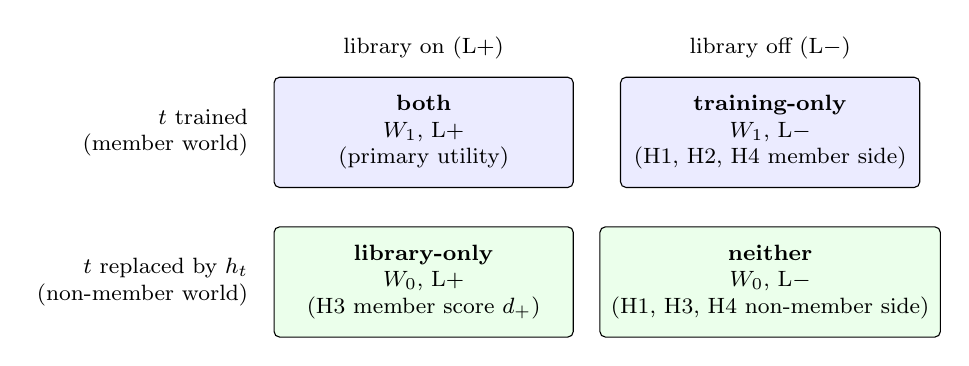
\begin{tikzpicture}
  \tikzset{cell/.style={box, minimum width=3.8cm, minimum height=1.4cm}}
  \node[cell, fill=blue!8]  (both)  at (0,0)    {\textbf{both}\\$W_1$, L+\\(primary utility)};
  \node[cell, fill=blue!8]  (train) at (4.4,0)  {\textbf{training-only}\\$W_1$, L$-$\\(H1, H2, H4 member side)};
  \node[cell, fill=green!8] (lib)   at (0,-1.9) {\textbf{library-only}\\$W_0$, L+\\(H3 member score $d_+$)};
  \node[cell, fill=green!8] (none)  at (4.4,-1.9) {\textbf{neither}\\$W_0$, L$-$\\(H1, H3, H4 non-member side)};
  \node[font=\footnotesize, above=1mm of both]  {library on (L+)};
  \node[font=\footnotesize, above=1mm of train] {library off (L$-$)};
  \node[font=\footnotesize, left=2mm of both, align=right] {$t$ trained\\(member world)};
  \node[font=\footnotesize, left=2mm of lib, align=right] {$t$ replaced by $h_t$\\(non-member world)};
\end{tikzpicture}
\caption{The four-cell design. A change of row needs a new federated training with the same seed and the same other records. A change of column only changes the content of one library slot, without retraining.}\label{fig:cells}
\end{figure}

\subsection{Threat model and leakage channels}\label{sec:threat}

We consider three adversaries. Each adversary sees a different object.
\begin{itemize}
  \item \textbf{Weights.} An auditor has the final model and the pretrained model. The auditor scores a known candidate record.
  \item \textbf{Client updates.} A malicious server knows a public candidate record. It changes the weights that it sends to the victim client and reads the returned gradient. This position follows the active attack of \citet{nguyen2023active}.
  \item \textbf{Datastore.} A RAG user sends ordinary questions about a candidate document and reads the answers.
\end{itemize}
All attacks are membership inference on a candidate that the adversary knows. None of them is an extraction attack.

\subsection{Notation}

Table~\ref{tab:notation} gives the notation. Each symbol has one meaning in all sections.

\begin{table}[tbp]
\centering
\small
\caption{Notation.}\label{tab:notation}
\begin{tabular}{@{}L{0.20\textwidth}L{0.55\textwidth}L{0.18\textwidth}@{}}
\toprule
Symbol & Meaning & Main use \\
\midrule
$K$, $k$, $R$, $S_r$ & Number of clients, client index, number of rounds, clients in round $r$. & FL \\
$\theta$, $\phi$ & Final federated model and pretrained reference model. & All attacks \\
$t=(c_t,q_t,a_t)$, $h_t$ & Target record (passage, training question, answer) and its held-out replacement. & Game \\
$W_1$, $W_0$ & Member world and non-member world. & Game \\
L+, L$-$ & Target passage in the library and not in the library. & Game \\
$\mathcal L$, $C_k(q)$, $T(q,c)$ & Library, top-$k$ retrieved passages, prompt template. & RAG \\
$\ell_{\theta,t}(x)$, $\bar\ell_\theta(x)$ & Per-token and mean negative log-likelihood (NLL). & Scores \\
$s(t,W)$ & Reference score of $t$ under world $W$. & H1 \\
$B$, $G(B)$, $d$ & Victim batch, returned batch gradient, target direction. & H2 \\
$(\tilde q_i,\tilde a_i)_{i=1}^{3}$ & The three probe questions of a passage and their gold answers. & H3, H4 \\
$d_{+}$, $d_{-}$ & Document score with the target passage in and out of the library. & H3 \\
$r_t$, $R_{\mathrm{arm}}$ & Closed-book retention of one target and its mean over targets. & H4 \\
$\varepsilon$, $\delta$, $\sigma$, $\rho$ & Privacy budget, failure probability, noise multiplier, zCDP parameter. & DP \\
$\sigma_{\mathrm{obs}}$ & Noise multiplier of the client's release noise on a returned gradient. & H2 \\
$\mathrm{TPR}$, $\mathrm{FPR}$, $\mathrm{BA}$ & True-positive rate, false-positive rate, balanced accuracy. & Evaluation \\
\bottomrule
\end{tabular}
\end{table}

\subsection{Attack signals}\label{sec:signals}

\subsubsection{Reference attack (weights)}\label{sec:reference}

The Reference attack compares the federated model with the pretrained model \citep{carlini2021extracting}. For a scoring text $x$,
\begin{equation}
  s_{\mathrm{ref}}(x)=-\frac{\bar\ell_\theta(x)}{\bar\ell_\phi(x)}.
  \label{eq:reference}
\end{equation}
A larger value means that fine-tuning made $x$ more probable relative to the pretrained model. We use two scoring forms. The \emph{record} form scores the closed-book record text. The \emph{template} form scores the answer given the template and, for RG, the passage. We select one form per arm on tuning data (Section~\ref{sec:attacker-choice}). For target $t$, the member score is $s_1=s(t,W_1)$ and the non-member score is $s_0=s(t,W_0)$. The library does not change this score.

\subsubsection{Causal gradient-alignment attack (client updates)}\label{sec:causal}

In the active membership inference attack of \citet{nguyen2023active}, a dishonest server puts a target-selective neuron into the global model and reads membership from the client's returned gradient. A malicious neuron or probe head changes the model architecture, so a client that inspects the model it receives can detect it. We therefore use an architecture-preserving variant, the \emph{causal gradient-alignment} attack. This variant is our construction. It does not inherit the chosen-neuron guarantee of the source attack. The server knows a public candidate $x^\star$ and the post-FL model $\theta_R$. It applies bounded, normalized gradient ascent on the candidate's loss:
\begin{equation}
  \theta^{(i+1)}=\theta^{(i)}+\eta_p\,\frac{\nabla_\theta\ell(x^\star;\theta^{(i)})}{\bigl\|\nabla_\theta\ell(x^\star;\theta^{(i)})\bigr\|},
  \qquad \theta^{(0)}=\theta_R,\quad i=0,\ldots,N_p-1,
\end{equation}
with $N_p$ probe epochs and step size $\eta_p$. The server sends $\theta_{\mathrm{req}}=\theta^{(N_p)}$ to the victim. The victim returns the gradient of its batch loss, $G(B)=\nabla_\theta\ell(B;\theta_{\mathrm{req}})$. The server computes the target direction $d=\nabla_\theta\ell(x^\star;\theta_{\mathrm{req}})$ and the score
\begin{equation}
  s_{\cos}(B)=\frac{\langle G(B),d\rangle}{\|G(B)\|\,\|d\|}.
  \label{eq:causal}
\end{equation}
The cosine divides out the overall gradient size of the batch, which a plain projection $\langle G(B),d\rangle/\|d\|$ does not. We use the validated configuration: cosine score, $N_p=12$ and $\eta_p=0.005$ (Section~\ref{sec:battery}). In each trial pair, the member batch is the non-member batch with one record replaced by the target.

\paragraph{Release noise.} A client can protect what it returns. In the release-noise condition, the victim clips its whole returned gradient to norm $C$ and adds Gaussian noise before the release,
\begin{equation}
  \tilde G(B)=G(B)\,\min\!\left(1,\frac{C}{\|G(B)\|}\right)+\mathcal N\!\left(0,\sigma_{\mathrm{obs}}^2C^2I\right),
  \qquad C=1,\ \sigma_{\mathrm{obs}}=1,
  \label{eq:release-noise}
\end{equation}
with fresh noise for every release. The server then scores $\tilde G(B)$ in place of $G(B)$ in Equation~\eqref{eq:causal}. This is the H2 primary condition (Section~\ref{sec:res-stage1}).

\subsubsection{Datastore attacks}\label{sec:nq}

The verbatim yes/no attack of \citet{anderson2024membership} shows the passage and asks whether it is in the context. A verbatim probe is easy to detect, and retrieval-side defenses withhold it \citep{choi2025mirabel}. We therefore use two natural-question attacks. They ask ordinary questions about the document \citep{naseh2025riddle,nguyen2026menta}.

For a document $c$ with probes $(\tilde q_i,\tilde a_i)_{i=1}^{3}$, the RAG system returns $y_i$ for each probe. The two scorers use the same three responses:
\begin{align}
  \text{F1 scorer (adapted from Riddle Me This):}\quad & u_i=\Fone(y_i,\tilde a_i), \label{eq:nq-f1}\\
  \text{Entailment scorer (adapted from MEntA):}\quad & u_i=P_{\mathrm{NLI}}\!\left(\text{entail}\mid c,\ \texttt{Question: }\tilde q_i\ \texttt{Answer: }y_i\right). \label{eq:nq-nli}
\end{align}
A refusal scores $u_i=0$ in the primary analysis. The document score is the mean $\bar u(c)=\frac13\sum_i u_i$. The document is the unit, and probes are never counted as independent observations. For target $t$, both scores come from $W_0$: $d_{+}$ with $c_t$ in the library and $d_{-}$ with $c_t$ out of the library. The same passage in and out is the comparator, so the two scores are matched on difficulty.

\subsubsection{Closed-book passage-fact retention (weights)}\label{sec:retention}

The three probes of target $t$ ask about facts that are not in $(q_t,a_t)$ (Section~\ref{sec:data}). We ask them without retrieval, with the template $T(\tilde q_i,\varnothing)$. The per-world retention score is the mean token F1 over the three probes, with refusals at 0. The retention of target $t$ is
\begin{equation}
  r_t=\Fone_{\mathrm{cb}}(W_1)-\Fone_{\mathrm{cb}}(W_0),
  \qquad
  R_{\mathrm{arm}}=\frac1n\sum_{t}r_t,
  \qquad
  D_{\mathrm{H4}}=R_{\mathrm{RG}}-R_{\mathrm{CB\text{-}AO}}.
  \label{eq:retention}
\end{equation}
H4 needs both $R_{\mathrm{RG}}>0$ and $D_{\mathrm{H4}}>0$. The difference alone could be positive because the CB-AO answers became worse while RG kept nothing. These quantities measure factual retention directly. They are not membership scores.

\subsection{Differential privacy accounting}\label{sec:dp}

The DP arms use DP-SGD with per-example clipping and Gaussian noise at each local step \citep{abadi2016deep}, with the answer-only mask. Our accountant uses Gaussian zero-concentrated DP \citep{bun2016zcdp} with replace-one adjacency and no subsampling amplification. It counts all local steps of the busiest client. With clip norm $C$, the replace-one sensitivity is $2C$, so each step costs $\rho_{\mathrm{step}}=2/\sigma^2$. Over $S$ steps,
\begin{equation}
  \rho=\frac{2S}{\sigma^2},\qquad
  \varepsilon=\rho+2\sqrt{\rho\ln(1/\delta)},\qquad \delta=10^{-5}.
  \label{eq:zcdp}
\end{equation}
The target client holds 33 records. With batch size 2, one local epoch and three rounds, $S=\lceil 33/2\rceil\times1\times3=51$. Table~\ref{tab:sigma} gives the noise for each budget. The clip norm is $C=1$.

\begin{table}[htbp]
\centering
\caption{Matched DP budgets. RG and CB-AO have the same record counts, batch size and steps, so a matched $\varepsilon$ gives the same $\sigma$.}\label{tab:sigma}
\begin{tabular}{@{}rrl@{}}
\toprule
$\varepsilon$ & $\sigma$ & Use \\
\midrule
$\infty$ & 0 & No DP \\
64 & 1.91 & Secondary; pilot only \\
16 & 5.45 & Primary for H6 \\
\bottomrule
\end{tabular}
\end{table}

The guarantee applies only to the accounted training releases: the DP-SGD client updates in the three FL rounds and anything computed from them (aggregated models, final weights and Reference scores). The privacy unit is one training record. The guarantee does not cover the answers to the crafted requests of a malicious server, the RAG outputs or the library. The optional release noise on the causal attack has its own accounting. The accountant is conservative, because a record takes part in only 3 of the 51 steps. Each run records its accounted $\varepsilon$ for both worlds, and the analysis refuses to compare runs whose $\varepsilon$ differ. The pilot ran all three budgets. The confirmation runs $\varepsilon=\infty$ and $\varepsilon=16$ only (Section~\ref{sec:res-stage1}).

\subsection{Related work and position of this study}\label{sec:related}

\paragraph{Membership inference against LLMs.} Loss-based attacks use the generalization gap \citep{yeom2018privacy}. Calibrated attacks compare the target likelihood with a reference model or a compressor \citep{carlini2021extracting}, with neighbors \citep{mattern2023membership}, with a non-member prefix \citep{xie2024recall}, or with token-level statistics \citep{shi2024detecting,zhang2025minkpp}. Other attacks use generation \citep{kaneko2024sampling}, self-prompt references \citep{fu2024membership} or local windows \citep{chen2026window}. \citet{carlini2022first} argue that an evaluation must report the true-positive rate at a low false-positive rate. These attacks observe a centrally trained model. They do not consider a federated server or a retrieval library.

\paragraph{Membership inference in federated learning.} \citet{nguyen2023active} give an active attack in which a dishonest server plants a target-selective neuron, and evaluate it under local DP. \citet{nguyen2025theoretically} analyse such attacks against LDP-protected clients in federated vision models. ProjRes is a passive attack on federated LLMs that uses server-visible gradient subspaces \citep{deng2026projres}. FISGuard defends against this attack with a fixed public input subspace \citep{jiang2026fisguard}. These studies do not include RAG.

\paragraph{Privacy in RAG.} \citet{anderson2024membership} infer datastore membership from verbatim questions. Riddle Me This \citep{naseh2025riddle} and MEntA \citep{nguyen2026menta} use natural questions. Mirabel detects suspicious queries and hides the retrieved document \citep{choi2025mirabel}. \citet{zeng2024good} find that retrieval at inference time can reduce the output of memorized training data. \citet{fu2025ensemble} compare MIAs against fine-tuned and RAG systems and propose an inference-time defense. These studies do not include federated training or an active server.

\paragraph{Grounded and federated RAG training.} RA-DIT conditions the LLM on retrieved chunks and puts the loss on the output segment only \citep{lin2024radit}. RAFT trains models on documents, distractors and answers \citep{zhang2024raft}. FedRAG supports federated fine-tuning of RAG generators and retrievers \citep{fajardo2025fedrag}. FedE4RAG federates the retrieval embeddings with privacy protection \citep{mao2025fede4rag}. These studies do not run membership attacks on the three channels.

\paragraph{Position.} Table~\ref{tab:compare} compares the ingredients. Each earlier study covers a subset of FL, LLMs, RAG and membership inference. A targeted review found no study that combines grounded versus closed-book federated training, an active-server update attack, a training-record audit, a datastore audit and matched DP budgets in one system. The review was not systematic, so we make no priority claim.

\begin{table}[htbp]
\centering
\caption{Ingredients of related studies, from the papers' stated methods. Upd.\ = attack or defense on client updates. Train = training-record membership. Store = datastore membership. Grd = grounded versus closed-book training.}\label{tab:compare}
\small
\begin{tabular}{@{}L{0.33\textwidth}*{7}{C{0.06\textwidth}}@{}}
\toprule
Study & FL & LLM & RAG & Train & Upd. & Store & Grd \\
\midrule
LLM MIAs \citep{yeom2018privacy,carlini2021extracting,shi2024detecting,zhang2025minkpp,mattern2023membership,xie2024recall,kaneko2024sampling,fu2024membership,chen2026window} & \no & \yes & \no & \yes & \no & \no & \no \\
Active MIA under LDP \citep{nguyen2023active,nguyen2025theoretically} & \yes & \no & \no & \no & \yes & \no & \no \\
ProjRes \citep{deng2026projres}, FISGuard \citep{jiang2026fisguard} & \yes & \yes & \no & \no & \yes & \no & \no \\
Verbatim and natural-question RAG MIAs \citep{anderson2024membership,naseh2025riddle,nguyen2026menta} & \no & \yes & \yes & \no & \no & \yes & \no \\
Mirabel \citep{choi2025mirabel} & \no & \yes & \yes & \no & \no & \yes & \no \\
Good and Bad of RAG \citep{zeng2024good} & \no & \yes & \yes & \yes & \no & \yes & \no \\
Ensemble Privacy Defense \citep{fu2025ensemble} & \no & \yes & \yes & \yes & \no & \yes & \no \\
RA-DIT \citep{lin2024radit}, RAFT \citep{zhang2024raft} & \no & \yes & \yes & \no & \no & \no & \yes \\
FedRAG \citep{fajardo2025fedrag} & \yes & \yes & \yes & \no & \no & \no & \yes \\
FedE4RAG \citep{mao2025fede4rag} & \yes & \no & \yes & \no & \no & \no & \no \\
\midrule
\textbf{This study} & \yes & \yes & \yes & \yes & \yes & \yes & \yes \\
\bottomrule
\end{tabular}
\end{table}

% ===========================================================================
\section{Experimental Setup}\label{sec:setup}
% ===========================================================================

\subsection{Research question and hypotheses}\label{sec:hyp}

\textbf{Main question.} When federated clients fine-tune with retrieved context (grounded training) instead of closed-book, how does private-information leakage change through each channel (the weights, the client updates and the datastore)? What is the cost in answer quality at matched, accounted privacy budgets?

Table~\ref{tab:hyp} gives the seven primary hypotheses. A hypothesis is ``supported'' only under the rules of Section~\ref{sec:stats}.

\begin{table}[tbp]
\centering
\small
\caption{Primary hypotheses.}\label{tab:hyp}
\begin{tabular}{@{}L{0.20\textwidth}L{0.42\textwidth}L{0.32\textwidth}@{}}
\toprule
Hypothesis & Statement & Primary endpoint \\
\midrule
H1 Weights: record membership & RG leaks less training-record membership than CB-AO, with acceptable RAG answer quality. & Reference pooled AUC (training-only vs neither); RAG F1 on F. \\
H2 Client updates & RG changes leakage through noise-protected client updates compared with CB-AO (two-sided). & Causal attack mean per-target AUC in $W_1$, release-noise pass ($\sigma_{\mathrm{obs}}=1$). \\
H3 Datastore & RG makes library documents more detectable than CB-AO. & Natural-question pooled AUC (library-only vs neither). \\
H4 Weights: passage-fact retention & RG stores facts from training passages that the training pair did not contain. & $R_{\mathrm{RG}}$ and $D_{\mathrm{H4}}$, both in F1. \\
H5 Is private training needed? & RG-public gives acceptable RAG answer quality relative to RG at $\varepsilon=\infty$. & RAG F1 on F. \\
H6 Utility at an equal budget & At $\varepsilon=16$, RG answers better than CB-AO, with training-record leakage no worse. & RAG F1 on F; Reference pooled AUC at $\varepsilon=16$. \\
H7 Is fine-tuning needed at all? & Without fine-tuning, RAG answer quality (P0) is non-inferior to RG at $\varepsilon=\infty$. & RAG F1 on F, margin 0.05, confirmation data only. \\
\bottomrule
\end{tabular}
\end{table}

\textbf{Cross-channel claim.} We claim a ``channel shift'' only if H1 is supported (weight leakage falls) \emph{and} either the H2 outcome is ``RG increases'' or H3 is supported. H4 is a second weights finding. It never counts toward a cross-channel claim. We never average channels.

\subsection{Selection of the attack battery}\label{sec:battery}

\paragraph{Screened attacks.} Before the main study, we adapted eleven published MIAs to federated fine-tuning: LOSS \citep{yeom2018privacy}, Reference and zlib \citep{carlini2021extracting}, Min-K\% \citep{shi2024detecting}, Min-K\%++ \citep{zhang2025minkpp}, Neighborhood \citep{mattern2023membership}, ReCaLL \citep{xie2024recall}, SaMIA \citep{kaneko2024sampling}, WBC \citep{chen2026window}, SPV-MIA \citep{fu2024membership} and the active attack AMIA \citep{nguyen2023active}. We screened them in a shared FL runner with DistilGPT2, SQuAD records of the form \texttt{Question: \ldots{} Answer: \ldots} with at most 64 tokens, and an attacker who scores records on the final FedAvg model only. We considered the other nine attacks and dropped them, because they did not fit this environment and gave no useful membership decisions:
\begin{itemize}
  \item \textbf{Min-K\%, Min-K\%++, Neighborhood, SaMIA, ReCaLL, zlib and LOSS.} These attacks were designed for long pretraining-style text scored on a centrally trained model. A short question--answer record gives few low-probability tokens (Min-K\%, Min-K\%++), a very short suffix for sampling (SaMIA) and little to compress (zlib). ReCaLL's non-member prefix is not in the record format. The signal of one record is also diluted in a FedAvg aggregate of four clients. Their fixed decision thresholds therefore gave one label to almost every record. For example, Min-K\% called every record a non-member in all 19 runs, and SaMIA did the same in all 16 runs. In the larger runs with 100 trials, Min-K\%, Min-K\%++, Neighborhood and zlib were close to chance (AUC 0.56--0.61). LOSS gave a weak signal (mean balanced accuracy 0.60).
  \item \textbf{WBC and SPV-MIA.} These attacks ranked members above non-members but had high false-positive rates (0.53 and 0.82). WBC needs the same access as the Reference attack, which performed better, so it adds no new channel. Our SPV-MIA adaptation could not reproduce the source's large self-prompted reference model at this scale.
\end{itemize}
The screening was a coarse filter with mostly six-trial runs on a small model. A dropped attack can work in another setting.

\paragraph{The kept attacks.} We kept the Reference attack for the weights. It had the best passive result in the screening (mean balanced accuracy 0.78 at a mean FPR of 0.04), and in a pilot on Qwen2.5-0.5B-Instruct it separated all 10 member/non-member pairs without DP. We kept the active-server attack for the client updates. AMIA was perfect in all 14 screening runs. Its malicious probe head changes the model architecture, however, and a client that checks the architecture of the model it receives rejects it. We therefore replaced the head with the architecture-preserving causal attack of Section~\ref{sec:causal}. A pre-registered validation of this attack on 10 fresh targets with 20 member/non-member pairs each gave a mean per-target AUC of 0.992 (95\% interval [0.981, 0.999]). The member batch scored higher in all 200 pairs. The validation also fixed the score: a projection score was unreliable (mean AUC 0.331 at 80 probe epochs), and the cosine score at 12 probe epochs was selected. The threshold calibrated on public batches at a 5\% FPR gave a 16.5\% FPR on private batches, so we use the threshold-free per-target AUC.

\paragraph{The datastore attacks.} Earlier pilots used the verbatim yes/no attack of \citet{anderson2024membership}. On our RAG system, it detected library membership (balanced accuracy 0.635 without DP), but mainly through a strong bias towards ``yes''. Verbatim probes are also easy to detect. Our verbatim-overlap gate withholds all of them (Section~\ref{sec:res-stage0}), and Mirabel targets them \citep{choi2025mirabel}. Mirabel itself was not usable in our system: at its default significance of 0.05, it removed the gold document for 81\% of benign questions. We therefore replaced the verbatim attack with the two natural-question attacks of Section~\ref{sec:nq} and keep it only as a baseline.

\subsection{System and implementation}\label{sec:framework}

Table~\ref{tab:stack} gives the experiment stack. All model and dataset revisions are pinned.

\begin{table}[tbp]
\centering
\small
\caption{Experiment stack.}\label{tab:stack}
\begin{tabular}{@{}L{0.25\textwidth}L{0.69\textwidth}@{}}
\toprule
Component & Setting \\
\midrule
FL framework & Flower simulation \citep{beutel2020flower} (\texttt{flwr[simulation]}, backed by Ray). FedAvg aggregation of full state dictionaries. One client trains at a time, so the four clients train in sequence in each round. \\
Generator LLM & \texttt{Qwen/Qwen2.5-0.5B-Instruct} \citep{qwen2025}, revision \texttt{7ae55760}. Full-parameter AdamW in FP32. The pretrained copy is the Reference model $\phi$. \\
Dataset & SQuAD v1.1 train split \citep{rajpurkar2016squad} (\texttt{rajpurkar/squad}), revision \texttt{7b6d24c4}. \\
FL setting & 4 clients, all 4 in each round, 3 rounds, 1 local epoch, batch size 2, client learning rate $2\times10^{-5}$, 32 base records per client. Maximum length 512 tokens, with no truncation of any training record. \\
Retriever & \texttt{sentence-transformers/all-MiniLM-L6-v2}, revision \texttt{1110a243}, mean pooling with L2 normalization; top-4 passages; at most 768 context tokens. \\
Generation & Qwen chat template; greedy decoding; at most 64 new tokens. \\
NLI model & \texttt{cross-encoder/nli-deberta-v3-base}, revision \texttt{6c749ce3} (entailment scorer). \\
Libraries & Hugging Face \texttt{transformers}, \texttt{datasets}, PyTorch, NumPy, scikit-learn. \\
Experiment control & Frozen launch files that pin the protocol, the study data and a hash of the code; CPU resolution of every target, world and token check before any GPU work; one job per process. \\
Hardware & One GPU per job on a Linux server; Python 3.10.12. \\
\bottomrule
\end{tabular}
\end{table}
% Add the GPU model and memory, CUDA, PyTorch and Flower versions of the server to the Hardware row.

\paragraph{Pre-registration.} The Stage~0 and Stage~1 procedures were frozen in a protocol file before any GPU job ran. The tool refuses to run a launch whose protocol is not frozen. The Stage~2 protocol was frozen after the pilot and before any confirmation job. Its definitions, margins and rules can become stricter than in Stage~1, but never less strict, and any other change needs a new pre-registration. One such change was made: the H2 primary endpoint moved to the release-noise pass after the pilot (Section~\ref{sec:res-stage1}). The analysis step applies the fixed rules once, and it was run once, after the last confirmation job. The integrity check that runs before it reports only row counts, accounted budgets and timings, never an endpoint value.

\paragraph{Observation rounds of the causal attack.} The crafted request goes only to the attacked client. That client receives the same partition, seeds and request as in a full round, so its returned gradient is unchanged. The three other clients take no part in the observation rounds. The victim's returned gradient is computed in the job's own process, with the request loaded once per pass, and the release noise is drawn on the GPU. The server still sees only the released arrays. A test on a small model shows that this path releases bit-identical gradients and gives identical trial records to the path through the Flower client.

\paragraph{Non-determinism.} GPU training is not bit-reproducible. Two runs of the same target and seed gave the same round-1 training loss (1.42352) but different round-3 losses (0.422 and 0.326), and the causal attack amplified the difference. We therefore treat each world as one random draw, as the paired design assumes. The noise affects $W_1$ and $W_0$ alike, and the target bootstrap carries it into the intervals.

\subsection{How RAG is used in the setup}\label{sec:rag-setup}

RAG enters the study at two points: in training (RG arms) and at answer time (all arms). Figure~\ref{fig:system} shows the full system, and Figure~\ref{fig:records} shows the training records.

\paragraph{Training.} In the RG and RG-public arms, each client record is a triple $(c,q,a)$. The client puts the passage $c$ in the context slot of the same prompt template that the RAG system uses at answer time (Qwen chat format). The loss is on the answer tokens and the end-of-turn token only (Equation~\eqref{eq:rg}). In CB-AO, the template is the same but the context slot is empty. Training uses the gold SQuAD passage, not a retrieved passage. This is an oracle-context condition.

\paragraph{Answer time.} The RAG system encodes the question with the frozen MiniLM encoder, ranks the library passages by cosine similarity and keeps the top four. It joins them into the context slot, with at most 768 context tokens. The generator then answers with at most 64 new tokens. The template is:
\begin{center}
\fbox{\begin{minipage}{0.86\textwidth}\ttfamily\footnotesize
Use the context to answer the question.\\
Question: \{question\}\\
Context:\\
\{top-4 retrieved passages\}\\
Answer:
\end{minipage}}
\end{center}
The template is inside the model's native user turn, and the assistant turn follows.

\paragraph{The private library.} The private library $\mathcal L$ has 255 fixed passages and one slot. In L$-$, the slot holds a filler passage that no probe asks about. In L+, the slot holds the target passage. The library size is therefore 256 in both conditions. The utility set F has 300 questions about the fixed passages only. A public library P (256 passages) gives a secondary utility measure.

\paragraph{The verbatim-overlap gate.} We calibrate a library gate on CPU. The gate computes the share of the query's word 3-grams that occur verbatim in the top-ranked document. It withholds that document at or above a threshold $\tau$. The threshold is the smallest value on a grid from 0.05 to 1.00 with at most 5\% benign gold-document loss. In the paired jobs, we record the gate decision only. The gate does not change the answer and triggers no extra generation.

\begin{figure}[tbp]
\centering
\resizebox{\textwidth}{!}{%
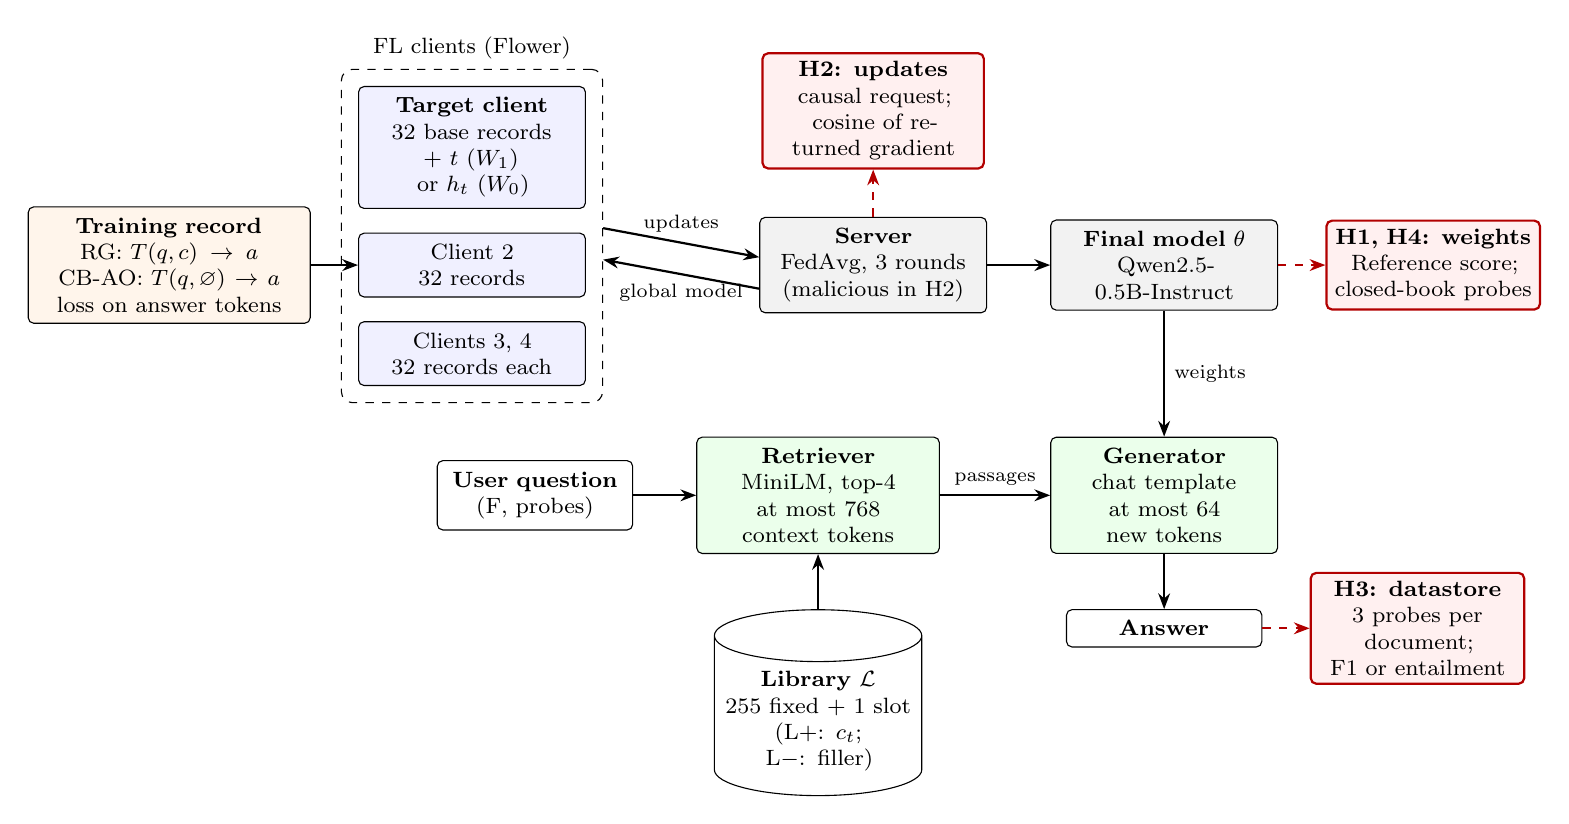
\begin{tikzpicture}[node distance=5mm and 6mm]
  % clients
  \node[box, text width=2.6cm, fill=blue!6] (c0) {\textbf{Target client}\\32 base records\\+ $t$ ($W_1$) or $h_t$ ($W_0$)};
  \node[box, text width=2.6cm, fill=blue!6, below=3mm of c0] (c1) {Client 2\\32 records};
  \node[box, text width=2.6cm, fill=blue!6, below=3mm of c1] (c2) {Clients 3, 4\\32 records each};
  \node[grp, fit=(c0)(c1)(c2), label={[font=\footnotesize]above:FL clients (Flower)}] (clients) {};
  % record format
  \node[box, text width=3.3cm, left=6mm of c1, fill=orange!8] (fmt) {\textbf{Training record}\\RG: $T(q,c)\rightarrow a$\\CB-AO: $T(q,\varnothing)\rightarrow a$\\loss on answer tokens};
  \draw[flow] (fmt) -- (c1);
  % server
  \node[box, text width=2.6cm, right=22mm of c1, fill=gray!10] (server) {\textbf{Server}\\FedAvg, 3 rounds\\(malicious in H2)};
  \draw[flow] ([yshift=1mm]clients.east) -- node[above, font=\scriptsize]{updates} ([yshift=1mm]server.west);
  \draw[flow] ([yshift=-3mm]server.west) -- node[below, font=\scriptsize]{global model} ([yshift=-3mm]clients.east);
  % model
  \node[box, text width=2.6cm, right=8mm of server, fill=gray!10] (model) {\textbf{Final model} $\theta$\\Qwen2.5-0.5B-Instruct};
  \draw[flow] (server) -- (model);
  % RAG
  \node[box, text width=2.6cm, below=16mm of model, fill=green!8] (gen) {\textbf{Generator}\\chat template\\at most 64\\new tokens};
  \node[box, text width=2.8cm, left=14mm of gen, fill=green!8] (ret) {\textbf{Retriever}\\MiniLM, top-4\\at most 768\\context tokens};
  \node[store, text width=2.4cm, below=7mm of ret] (lib) {\textbf{Library} $\mathcal L$\\255 fixed + 1 slot\\(L+: $c_t$; L$-$: filler)};
  \node[box, text width=2.2cm, left=8mm of ret, fill=white] (user) {\textbf{User question}\\(F, probes)};
  \draw[flow] (user) -- (ret);
  \draw[flow] (lib) -- (ret);
  \draw[flow] (ret) -- node[above, font=\scriptsize]{passages} (gen);
  \draw[flow] (model) -- node[right, font=\scriptsize]{weights} (gen);
  \node[box, text width=2.2cm, below=7mm of gen] (ans) {\textbf{Answer}};
  \draw[flow] (gen) -- (ans);
  % attacks
  \node[atk, text width=2.5cm, right=6mm of model] (a1) {\textbf{H1, H4: weights}\\Reference score;\\closed-book probes};
  \node[atk, text width=2.6cm, above=6mm of server] (a2) {\textbf{H2: updates}\\causal request;\\cosine of returned gradient};
  \node[atk, text width=2.5cm, right=6mm of ans] (a3) {\textbf{H3: datastore}\\3 probes per document;\\F1 or entailment};
  \draw[leak] (model) -- (a1);
  \draw[leak] (server) -- (a2);
  \draw[leak] (ans) -- (a3);
\end{tikzpicture}%
}
\caption{The federated RAG system of the study and the three leakage channels. Black arrows are the normal data flow. Dashed red arrows show what each adversary observes.}\label{fig:system}
\end{figure}

\begin{figure}[tbp]
\centering
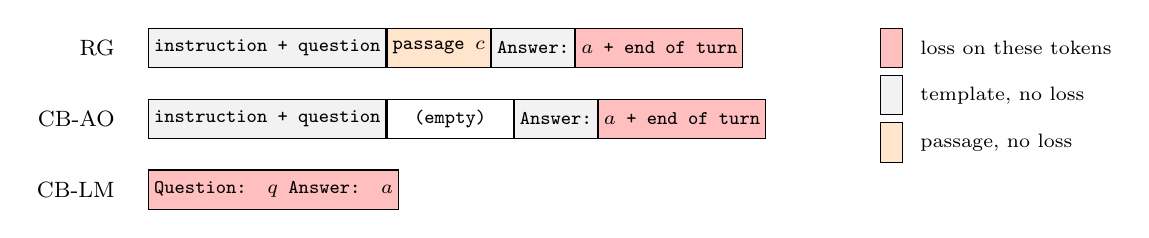
\begin{tikzpicture}[node distance=3mm]
  \tikzset{tok/.style={draw, font=\scriptsize\ttfamily, minimum height=5mm, inner sep=2pt}}
  % RG
  \node[font=\footnotesize, anchor=east] (lrg) at (0,0) {RG};
  \node[tok, anchor=west, fill=gray!10] (rg1) at (0.3,0) {instruction + question};
  \node[tok, right=0pt of rg1, fill=orange!20] (rg2) {passage $c$};
  \node[tok, right=0pt of rg2, fill=gray!10] (rg3) {Answer:};
  \node[tok, right=0pt of rg3, fill=red!25] (rg4) {$a$ + end of turn};
  % CB-AO
  \node[font=\footnotesize, anchor=east] (lcb) at (0,-0.9) {CB-AO};
  \node[tok, anchor=west, fill=gray!10] (cb1) at (0.3,-0.9) {instruction + question};
  \node[tok, right=0pt of cb1, fill=white, minimum width=1.6cm] (cb2) {(empty)};
  \node[tok, right=0pt of cb2, fill=gray!10] (cb3) {Answer:};
  \node[tok, right=0pt of cb3, fill=red!25] (cb4) {$a$ + end of turn};
  % CB-LM
  \node[font=\footnotesize, anchor=east] (llm) at (0,-1.8) {CB-LM};
  \node[tok, anchor=west, fill=red!25] (lm1) at (0.3,-1.8) {Question: $q$ Answer: $a$};
  % legend
  \node[tok, fill=red!25, anchor=west] (k1) at (9.6,0) {\phantom{x}};
  \node[font=\scriptsize, right=1mm of k1] {loss on these tokens};
  \node[tok, fill=gray!10, anchor=west] (k2) at (9.6,-0.6) {\phantom{x}};
  \node[font=\scriptsize, right=1mm of k2] {template, no loss};
  \node[tok, fill=orange!20, anchor=west] (k3) at (9.6,-1.2) {\phantom{x}};
  \node[font=\scriptsize, right=1mm of k3] {passage, no loss};
\end{tikzpicture}
\caption{Training-record formats. RG and CB-AO use the same chat template and the same answer-only loss. They differ only in the context slot. CB-LM is the conventional closed-book record, with the loss on all tokens.}\label{fig:records}
\end{figure}

\subsection{Data design}\label{sec:data}

The source is the SQuAD train split. The builder partitions it by article into groups (Table~\ref{tab:groups}). The groups do not share articles. The only exception is the target's own passage, which enters the private library in the L+ condition.

\begin{table}[tbp]
\centering
\small
\caption{Data groups (study seed 20260930).}\label{tab:groups}
\begin{tabular}{@{}L{0.10\textwidth}L{0.42\textwidth}L{0.42\textwidth}@{}}
\toprule
Group & Contents & Use \\
\midrule
T & (passage, question, answer), one question per passage; at least 600 passages. & Client data and target records. For each target seed, 128 base records from other articles; $W_1$ and $W_0$ share them. \\
T-hold & Same form. & The replacement $h_t$ in $W_0$. \\
U & Same form; at least 160 passages. & RG-public training. \\
L & 64 articles $\times$ 4 passages. & Private library; its questions form F (300 questions, at most 2 per passage). \\
N & 16 articles $\times$ 4 passages, never in a library. & Non-member documents for the secondary datastore AUC. \\
P & 32 articles $\times$ 8 passages. & Public library and public-library utility (100 questions). \\
V & A copy of the layout above, plus an attacker-calibration slice. & All tuning, validation and pilots. \\
\bottomrule
\end{tabular}
\end{table}

\paragraph{Target and probe eligibility.} The rules are fixed in advance and do not use outcomes.
\begin{itemize}
  \item A target passage needs at least four SQuAD questions and 24--160 words.
  \item The first question in seeded order is the training pair.
  \item The next three \emph{qualifying} siblings are the probes. A sibling qualifies only if its normalized gold answer does not occur in the training question or answer, the training answer does not occur in its gold answer, and its answer span does not overlap the training answer span.
  \item A passage with fewer than three qualifying siblings cannot be a target. The builder counts these skips.
  \item The builder excludes every question that served as a target in our earlier experiments, through recomputed record hashes, so that no target has been seen by an earlier attack.
  \item Every RG, CB-AO and CB-LM record must fit the maximum length without truncation, or the build stops.
\end{itemize}

\subsection{Arms}\label{sec:arms}

All training arms share the model, the FL setting, the questions, the prompt template and the answer-only loss (Table~\ref{tab:arms}). In the pilot, RG and CB-AO are each trained at $\varepsilon\in\{\infty,64,16\}$. In the confirmation, they are trained at $\varepsilon\in\{\infty,16\}$.

\begin{table}[tbp]
\centering
\small
\caption{Arms.}\label{tab:arms}
\begin{tabular}{@{}L{0.12\textwidth}L{0.24\textwidth}L{0.15\textwidth}L{0.12\textwidth}L{0.22\textwidth}@{}}
\toprule
Arm & Training data & Context slot & Loss & Unit \\
\midrule
RG & Private client triples & The passage & Answer only & Per target (paired worlds) \\
CB-AO & The same questions and answers & Empty & Answer only & Per target (paired worlds) \\
RG-public & Public triples (U) & The passage & Answer only & 5 seeds, shared by all targets \\
P0 & None (pretrained) & -- & -- & One model \\
CB-LM (bridge) & Closed-book records & Conventional format & Full LM & Pilot only \\
\bottomrule
\end{tabular}
\end{table}

\subsection{Measurement procedures}\label{sec:measure}

Figure~\ref{fig:attacks} shows the procedure of each attack.

\begin{figure}[tbp]
\centering
\resizebox{\textwidth}{!}{%
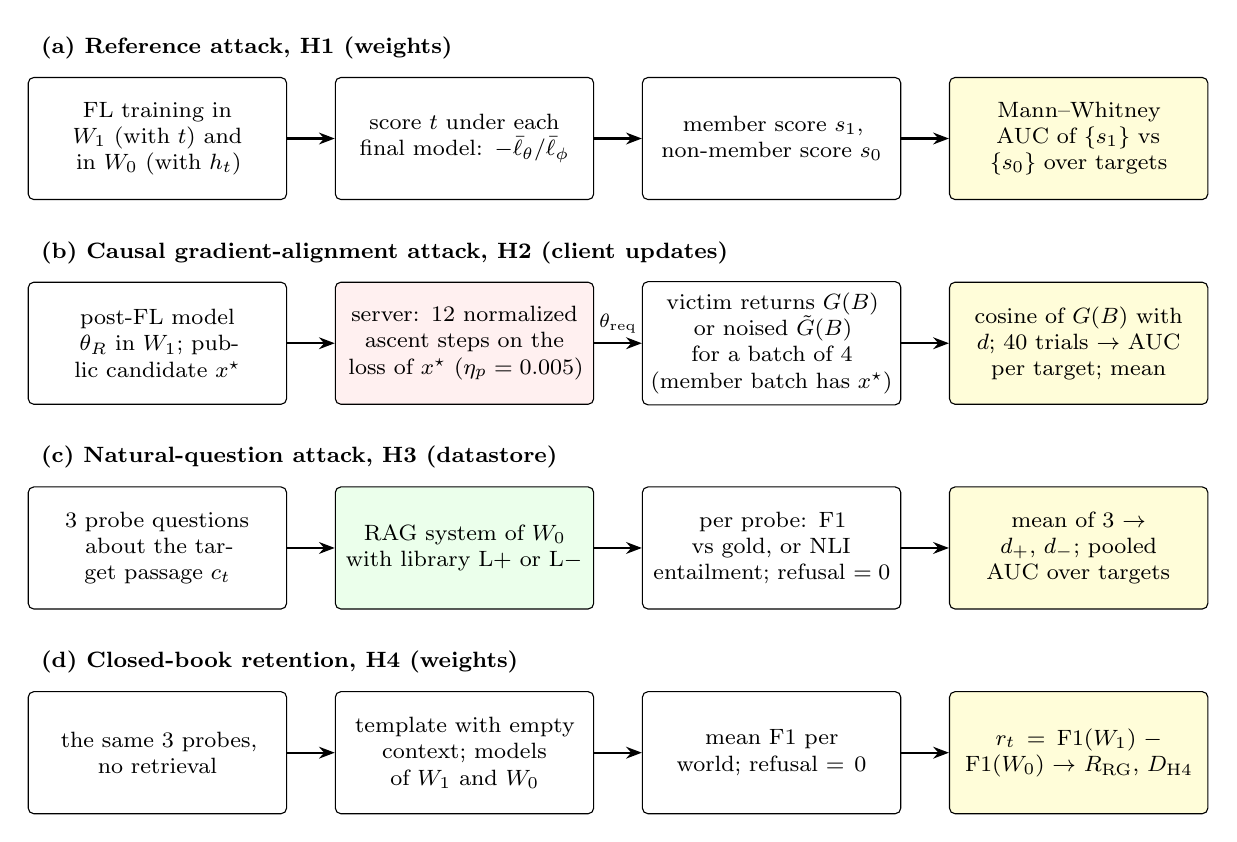
\begin{tikzpicture}
  \tikzset{st/.style={box, text width=3.0cm, minimum height=1.55cm},
           ep/.style={st, fill=yellow!15},
           ttl/.style={font=\footnotesize\bfseries, anchor=west}}
  \def\xa{0} \def\xb{3.9} \def\xc{7.8} \def\xd{11.7}
  % (a)
  \node[ttl] at (-1.6,1.15) {(a) Reference attack, H1 (weights)};
  \node[st] (a1) at (\xa,0) {FL training in $W_1$ (with $t$) and in $W_0$ (with $h_t$)};
  \node[st] (a2) at (\xb,0) {score $t$ under each final model: $-\bar\ell_\theta/\bar\ell_\phi$};
  \node[st] (a3) at (\xc,0) {member score $s_1$, non-member score $s_0$};
  \node[ep] (a4) at (\xd,0) {Mann--Whitney AUC of $\{s_1\}$ vs $\{s_0\}$ over targets};
  \draw[flow] (a1) -- (a2); \draw[flow] (a2) -- (a3); \draw[flow] (a3) -- (a4);
  % (b)
  \node[ttl] at (-1.6,-1.45) {(b) Causal gradient-alignment attack, H2 (client updates)};
  \node[st] (b1) at (\xa,-2.6) {post-FL model $\theta_R$ in $W_1$; public candidate $x^\star$};
  \node[st, fill=red!6] (b2) at (\xb,-2.6) {server: 12 normalized ascent steps on the loss of $x^\star$ ($\eta_p=0.005$)};
  \node[st] (b3) at (\xc,-2.6) {victim returns $G(B)$ or noised $\tilde G(B)$ for a batch of 4 (member batch has $x^\star$)};
  \node[ep] (b4) at (\xd,-2.6) {cosine of $G(B)$ with $d$; 40 trials $\rightarrow$ AUC per target; mean};
  \draw[flow] (b1) -- (b2); \draw[flow] (b2) -- node[above, font=\scriptsize]{$\theta_{\mathrm{req}}$} (b3); \draw[flow] (b3) -- (b4);
  % (c)
  \node[ttl] at (-1.6,-4.05) {(c) Natural-question attack, H3 (datastore)};
  \node[st] (c1) at (\xa,-5.2) {3 probe questions about the target passage $c_t$};
  \node[st, fill=green!8] (c2) at (\xb,-5.2) {RAG system of $W_0$ with library L+ or L$-$};
  \node[st] (c3) at (\xc,-5.2) {per probe: F1 vs gold, or NLI entailment; refusal $=0$};
  \node[ep] (c4) at (\xd,-5.2) {mean of 3 $\rightarrow$ $d_+$, $d_-$; pooled AUC over targets};
  \draw[flow] (c1) -- (c2); \draw[flow] (c2) -- (c3); \draw[flow] (c3) -- (c4);
  % (d)
  \node[ttl] at (-1.6,-6.65) {(d) Closed-book retention, H4 (weights)};
  \node[st] (d1) at (\xa,-7.8) {the same 3 probes, no retrieval};
  \node[st] (d2) at (\xb,-7.8) {template with empty context; models of $W_1$ and $W_0$};
  \node[st] (d3) at (\xc,-7.8) {mean F1 per world; refusal $=0$};
  \node[ep] (d4) at (\xd,-7.8) {$r_t=\Fone(W_1)-\Fone(W_0)$ $\rightarrow$ $R_{\mathrm{RG}}$, $D_{\mathrm{H4}}$};
  \draw[flow] (d1) -- (d2); \draw[flow] (d2) -- (d3); \draw[flow] (d3) -- (d4);
\end{tikzpicture}%
}
\caption{The attack procedures. Yellow boxes are the primary endpoints.}\label{fig:attacks}
\end{figure}

\paragraph{H1: Reference.} For each target, we compute $s_1$ and $s_0$ (Section~\ref{sec:reference}). The pooled AUC per arm is the Mann--Whitney AUC of $\{s_1\}$ against $\{s_0\}$ over the $n$ targets:
\begin{equation}
  \AUC=\frac{1}{n_1n_0}\sum_{i}\sum_{j}\Bigl(\ind[s_{1,i}>s_{0,j}]+\tfrac12\,\ind[s_{1,i}=s_{0,j}]\Bigr).
  \label{eq:mw}
\end{equation}

\paragraph{H2: causal attack.} We use the validated configuration (cosine score, $N_p=12$, $\eta_p=0.005$). Each pass runs 40 trials (20 counterbalanced member/non-member batch pairs) in $W_1$ only. We compute the AUC per target and report the mean over targets. The attacker's loss direction (the record LM loss, or the answer-only loss given the template and passage) is fixed per arm on tuning data. Each job runs two passes on the same $W_1$: a plain pass and a release-noise pass with $\sigma_{\mathrm{obs}}=1$ and $C=1$ (Equation~\eqref{eq:release-noise}). The release-noise pass is the H2 primary endpoint, and the plain pass is a reported secondary. The release noise has its own per-release accounting, which is never merged with the training $\varepsilon$.

\paragraph{H3: natural-question attack.} We ask three queries per document per condition, with retrieval on (Section~\ref{sec:nq}). We compute the pooled AUC of $\{d_+\}$ against $\{d_-\}$ over targets with Equation~\eqref{eq:mw}. A secondary AUC compares the inserted target passages with the N documents. As a baseline, we also ask one verbatim yes/no query per document and condition, outside the three-query budget.

\paragraph{H4: retention.} We ask the three probes without retrieval in $W_1$ and $W_0$ and compute Equation~\eqref{eq:retention}.

\paragraph{Utility.} The primary utility is the RAG token F1 on F (private library, retrieval on, top-4). We measure it on each $W_1$ with L+ and also score $W_0$. RG-public and P0 are scored on the same F. Secondary measures are exact match, public-library F1, no-context F1 and answer NLL.

\subsubsection{Attacker choices on tuning data}\label{sec:attacker-choice}

For each arm, we fix the Reference form, the causal direction and the H3 scorer on the tuning cohort (V, seeds 8000--8099). Each arm's choice pools that arm's pilot jobs over the three privacy budgets. The choice with the highest pooled tuning AUC wins. Ties go to the record form or to the F1 scorer. Only datastore scorers that pass the Stage~0 sensitivity check are eligible. The choices are frozen in the Stage~2 protocol (Table~\ref{tab:choices}). The confirmation jobs record both Reference forms and both scorers, but only the frozen choice decides, and they run the causal attack in the frozen direction only.

\subsection{Study stages}\label{sec:stages}

The study runs in three pre-registered stages (Figure~\ref{fig:stages}). Stage~0 validates the instruments, Stage~1 tunes the attacker on validation data, and Stage~2 tests the hypotheses on fresh targets.

\begin{figure}[tbp]
\centering
\resizebox{\textwidth}{!}{%
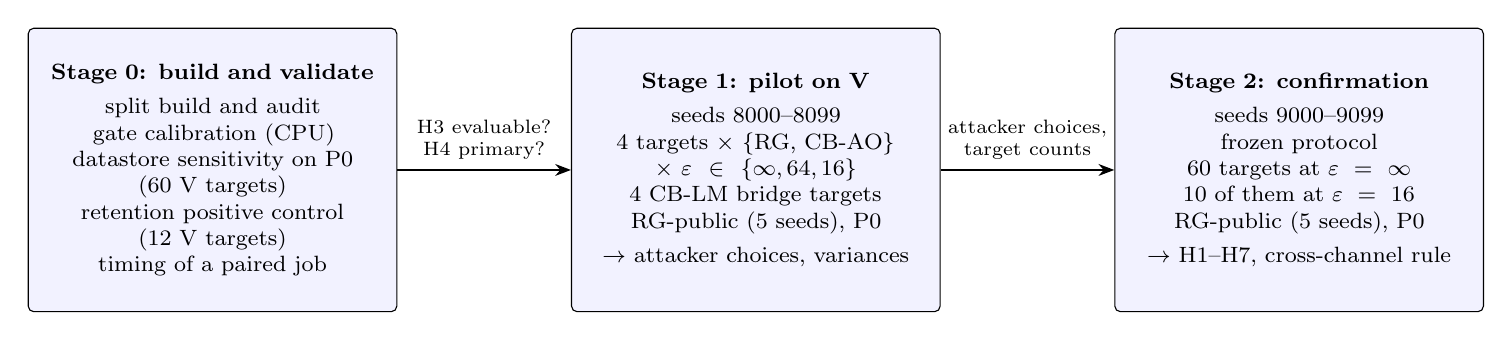
\begin{tikzpicture}
  \tikzset{stg/.style={box, text width=4.4cm, minimum height=3.6cm, anchor=north}}
  \node[stg, fill=blue!5] (s0) at (0,0) {\textbf{Stage 0: build and validate}\\[3pt]
    split build and audit\\
    gate calibration (CPU)\\
    datastore sensitivity on P0\\(60 V targets)\\
    retention positive control\\(12 V targets)\\
    timing of a paired job};
  \node[stg, fill=blue!5] (s1) at (6.9,0) {\textbf{Stage 1: pilot on V}\\[3pt]
    seeds 8000--8099\\
    4 targets $\times$ \{RG, CB-AO\}\\$\times$ $\varepsilon\in\{\infty,64,16\}$\\
    4 CB-LM bridge targets\\
    RG-public (5 seeds), P0\\[3pt]
    $\rightarrow$ attacker choices, variances};
  \node[stg, fill=blue!5] (s2) at (13.8,0) {\textbf{Stage 2: confirmation}\\[3pt]
    seeds 9000--9099\\
    frozen protocol\\
    60 targets at $\varepsilon=\infty$\\
    10 of them at $\varepsilon=16$\\
    RG-public (5 seeds), P0\\[3pt]
    $\rightarrow$ H1--H7, cross-channel rule};
  \draw[flow] (s0) -- node[above, font=\scriptsize, align=center]{H3 evaluable?\\H4 primary?} (s1);
  \draw[flow] (s1) -- node[above, font=\scriptsize, align=center]{attacker choices,\\target counts} (s2);
\end{tikzpicture}%
}
\caption{The three stages of the study. Validation and pilot data (V) are tuning data and are never reported as evidence for a hypothesis.}\label{fig:stages}
\end{figure}

\paragraph{Stage 0 (build and validate).} Stage~0 has these items:
\begin{enumerate}
  \item The split builder and its audit, with skip counts.
  \item The record encoders, the answer-only mask in both training paths (AdamW and DP-SGD) and prompt-parity tests.
  \item \textbf{Datastore sensitivity (H3).} P0, at least 60 V target passages, library in against out. A scorer passes if the 95\% bootstrap lower bound of its pooled AUC is at least 0.70. Only passing scorers are eligible. If no scorer passes, H3 is not evaluable.
  \item \textbf{Retention sensitivity (H4), a deliberate-memorization positive control.} Paired worlds on 12 V targets. After FL (RG, $\varepsilon=\infty$), the member world gets a central AdamW fine-tune on the plain passage text (full LM loss, one step per epoch, learning rate $10^{-4}$, 3 epochs).
  \begin{enumerate}
    \item \emph{Learning check, first and independent of the probes.} A target has learned its passage if its passage-token NLL in $W_1$ is at most $0.5\times$ that in $W_0$, and greedy continuation reproduces at least 50\% of the next 32 passage tokens given the first 32 \citep{biderman2023emergent}. If fewer than 10 of 12 targets learn, the control runs once more at 6 epochs. If fewer than 10 still learn, H4 becomes secondary (six primaries, 99.2\% intervals).
    \item \emph{Retention sensitivity (decisive).} On the learned targets, the mean $r_t$ must have a 95\% target-bootstrap lower bound above 0.05 F1.
    \item \emph{Membership-AUC sensitivity (secondary only).} On the learned targets, the training-only natural-question AUC lower bound must be at least 0.60. A failure never changes the primary status of H4.
  \end{enumerate}
  \item Gate calibration on V (CPU): at most 5\% benign gold-document loss.
  \item Timing of a full paired job, with and without DP-SGD.
\end{enumerate}

\paragraph{Stage 1 (pilot on V, seeds 8000--8099).} The pilot runs 4 targets $\times$ \{RG, CB-AO\} $\times$ $\varepsilon\in\{\infty,64,16\}$, plus 4 CB-LM bridge targets, RG-public (5 seeds) and P0. It fixes the attacker choices, estimates variances and projects the decision-interval half-widths of the confirmation. Pilot data are tuning data and are never reported as evidence. The pilot can tighten the design, but it cannot loosen it. In particular, the pilot's RG-versus-P0 difference is descriptive, and only H7 on the confirmation data decides whether fine-tuning is needed.

\paragraph{Stage 2 (confirmation, seeds 9000--9099).} The confirmation is paired: every target runs under every per-target arm. It uses the first 60 of the 124 eligible final targets for RG and CB-AO at $\varepsilon=\infty$, and the first 10 of these for RG and CB-AO at $\varepsilon=16$, with seed $9000+{}$target index. These are 140 paired jobs. RG-public (5 seeds, 9095--9099) and P0 are scored on the final F, which gives 146 jobs in total. No target of the confirmation was used in Stage~0 or Stage~1. The $\varepsilon=64$ budget of the pilot was not run. Each arm uses its frozen attacker choices (Table~\ref{tab:choices}), and the H2 primary endpoint is the release-noise pass, with the plain pass as a reported secondary. Section~\ref{sec:res-stage1} gives the reasons for the target counts, the budgets and the H2 endpoint.

\subsection{Statistics}\label{sec:stats}

\paragraph{Unit and intervals.} The target is the unit. Each target gives one Reference score pair, one causal AUC, one document score pair, one retention value and one utility value per world. For per-target endpoints, we use a paired target bootstrap with 10{,}000 resamples and the NumPy generator \texttt{default\_rng} with seed 20260930. Each resample carries all quantities of a target for all arms together, so arm differences are paired. Utility endpoints use a crossed cluster bootstrap. Each resample draws models (targets or seeds) and SQuAD article clusters of F independently, so that sibling questions stay together. H5 and H7 draw RG-public seeds, RG targets and article clusters independently.

\paragraph{Multiplicity.} There are seven primary hypotheses. Decision intervals are 99.3\% ($1-0.05/7$, Bonferroni). We also report 95\% intervals.

\paragraph{Outcome classification.} For a difference $D$, oriented so that a positive value is the direction of the hypothesis, with decision interval $[\mathrm{lo},\mathrm{hi}]$ and margin $m$ (0.05 AUC for attacks; 0.05 F1 for utility and H4), the first matching row of Table~\ref{tab:outcomes} gives the outcome.

\begin{table}[htbp]
\centering
\caption{Outcome classification (first match wins).}\label{tab:outcomes}
\begin{tabular}{@{}cll@{}}
\toprule
\# & Condition & Outcome \\
\midrule
1 & $\mathrm{lo}\geq m$ & Meaningful improvement \\
2 & $\mathrm{lo}>0$ & Statistical improvement, not shown to be meaningful \\
3 & $\mathrm{hi}\leq -m$ & Meaningful harm \\
4 & $\mathrm{hi}<0$ & Statistical harm, not shown to be meaningful \\
5 & $-m<\mathrm{lo}$ and $\mathrm{hi}<m$ & Equivalent within $\pm m$ \\
6 & otherwise & Inconclusive \\
\bottomrule
\end{tabular}
\end{table}

``Supported'' means outcome 1 or 2. ``Acceptable utility'' means $\mathrm{lo}>-0.05$. H2 is two-sided with $D=\AUC(\text{CB-AO})-\AUC(\text{RG})$: outcomes 1--2 read ``RG reduces'', 3--4 ``RG increases'', 5 ``no meaningful change'' and 6 ``inconclusive''. For H7, $D=\Fone(\text{P0})-\Fone(\text{RG},\varepsilon=\infty)$ on the confirmation data. If $\mathrm{lo}>-0.05$, fine-tuning is not needed for answer quality in this setting. If $\mathrm{hi}<-0.05$, RG is meaningfully better. Otherwise, H7 is inconclusive. A failure to show that RG beats P0 is never reported as ``fine-tuning unnecessary''.

% ===========================================================================
\section{Results}\label{sec:results}
% ===========================================================================

This section gives the Stage~0 validation results, the Stage~1 pilot results and the Stage~2 confirmation results. Stage~0 and Stage~1 use validation data (V). They establish that the instruments are sensitive, fix the attacker and size the confirmation. They are not evidence for or against a hypothesis. Only the Stage~2 confirmation on fresh final targets decides the hypotheses.

\subsection{Stage 0: build and validation}\label{sec:res-stage0}

\paragraph{Build.} All 50 targets of our earlier experiments matched SQuAD rows and were excluded. The builder removed 52 further questions, because SQuAD repeats some identical question--answer pairs. It skipped 2{,}972 passages outside 24--160 words and 174 duplicate questions within a passage. Table~\ref{tab:build} gives the eligible targets and the skips. One grounded training record of a 160-word passage needs 405 tokens, so the maximum length is 512 tokens. In the timing jobs, the longest training record had 329 tokens (mean 199).

\begin{table}[htbp]
\centering
\caption{Stage 0 build: eligible targets and skip counts.}\label{tab:build}
\small
\begin{tabular}{@{}lrrrr@{}}
\toprule
Cohort & Targets & Fewer than 4 questions & Fewer than 3 qualifying probes & Eligible, no hold record \\
\midrule
V & 186 & 63 & 55 & 311 \\
Final & 124 & 123 & 35 & 362 \\
\bottomrule
\end{tabular}
\end{table}

\paragraph{Gate calibration (CPU, V).} The selected threshold is $\tau=0.45$ (3-gram overlap with the top document). The benign gold-document loss is 4.4\% (13 of the 297 V utility questions whose gold document is retrieved), within the 5\% limit. The gate withholds the verbatim membership probes in 100\% of cases.

\paragraph{Datastore sensitivity (P0, 60 V targets).} Both scorers passed (Table~\ref{tab:ds}, Figure~\ref{fig:ds}). H3 is therefore evaluable, and both scorers are eligible for the attacker choice. The verbatim yes/no baseline had AUC 0.75. No refusals occurred, so the refusal-excluded AUCs equal the primary AUCs. This result validates the sensitivity of the attack on the pretrained model. It is not a privacy result.

\begin{table}[htbp]
\centering
\caption{Stage 0 datastore-sensitivity check on P0 (60 V targets; 95\% target-bootstrap intervals). The pass rule is a lower bound of at least 0.70.}\label{tab:ds}
\small
\begin{tabular}{@{}lllc@{}}
\toprule
Scorer & Pooled AUC, same passage in vs out & AUC vs 64 N documents (secondary) & Pass \\
\midrule
F1 & 0.902 [0.854, 0.947] & 0.890 [0.826, 0.945] & yes \\
Entailment & 0.887 [0.837, 0.934] & 0.907 [0.852, 0.953] & yes \\
\bottomrule
\end{tabular}
\end{table}

\begin{figure}[tbp]
\centering
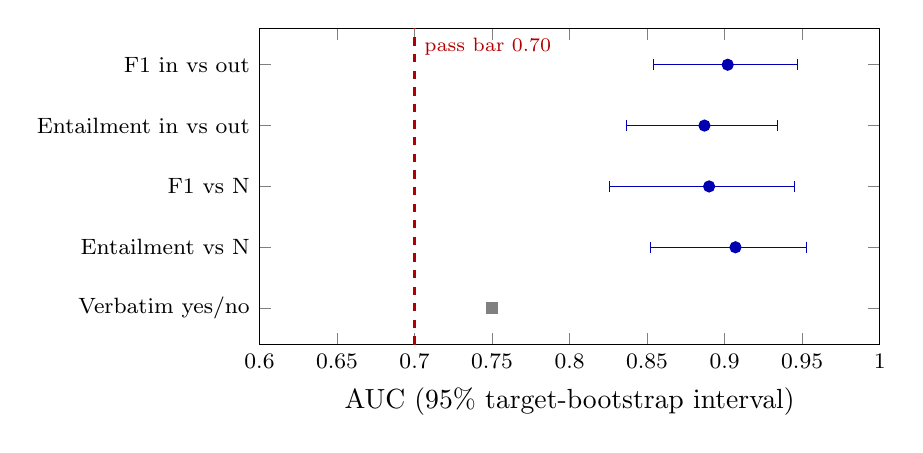
\begin{tikzpicture}
\begin{axis}[
  width=0.78\textwidth, height=5.6cm,
  xmin=0.6, xmax=1.0, xlabel={AUC (95\% target-bootstrap interval)},
  symbolic y coords={Verbatim yes/no,Entailment vs N,F1 vs N,Entailment in vs out,F1 in vs out},
  ytick={Verbatim yes/no,Entailment vs N,F1 vs N,Entailment in vs out,F1 in vs out},
  y tick label style={font=\footnotesize}, x tick label style={font=\footnotesize},
  enlarge y limits=0.15,
]
\addplot[only marks, mark=*, blue!70!black,
  error bars/.cd, x dir=both, x explicit] coordinates {
  (0.902,F1 in vs out) += (0.045,0) -= (0.048,0)
  (0.887,Entailment in vs out) += (0.047,0) -= (0.050,0)
  (0.890,F1 vs N) += (0.055,0) -= (0.064,0)
  (0.907,Entailment vs N) += (0.046,0) -= (0.055,0)};
\addplot[only marks, mark=square*, gray] coordinates {(0.75,Verbatim yes/no)};
\draw[dashed, thick, red!70!black] (rel axis cs:0.25,0) -- (rel axis cs:0.25,1);
\node[font=\scriptsize, red!70!black, anchor=north west] at (rel axis cs:0.25,1) {pass bar 0.70};
\end{axis}
\end{tikzpicture}
\caption{Stage 0 datastore-sensitivity check on the pretrained model P0. The pass rule applies to the lower bound of the ``in vs out'' AUC. The verbatim baseline is a point estimate.}\label{fig:ds}
\end{figure}

\paragraph{Retention positive control (12 V targets).} At 3 epochs, only 4 of 12 targets learned their passage, below the required 10. By the pre-registered rule, the control ran once more at 6 epochs on the same 12 targets. At 6 epochs, 10 of 12 targets learned their passage, which meets the rule. Table~\ref{tab:control} gives the results. The ten learned targets had a passage-NLL ratio between 0.000 and 0.106 and reproduced all 32 continuation tokens. The two other targets passed the NLL criterion (0.138 and 0.031) but failed the continuation criterion (0.375 and 0.188). On the learned targets, the mean retention was $0.142$ F1 with 95\% interval $[0.066, 0.225]$. The lower bound is above 0.05, so the retention probes are sensitive, and H4 stays primary. There are therefore seven primary hypotheses with 99.3\% decision intervals. The secondary membership AUCs in the training-only cell were also sensitive. This control shows that the probes detect deliberately memorized passage facts. It is not a finding about grounded training.

\begin{table}[htbp]
\centering
\caption{Stage 0 retention positive control (RG, $\varepsilon=\infty$, plus a central fine-tune of the member world on the passage text; 95\% target-bootstrap intervals on the learned targets).}\label{tab:control}
\small
\begin{tabular}{@{}lll@{}}
\toprule
Quantity & Result & Rule \\
\midrule
Learned targets, 3 epochs & 4 of 12 & $\geq 10$; failed, one rerun \\
Learned targets, 6 epochs & 10 of 12 & $\geq 10$; passed \\
Mean retention $r_t$ (learned targets) & 0.142 [0.066, 0.225] & lower bound $>0.05$; passed \\
Training-only NQ AUC, F1 scorer (secondary) & 0.80 [0.65, 0.95] & lower bound $\geq 0.60$; passed \\
Training-only NQ AUC, entailment scorer (secondary) & 0.95 [0.87, 1.00] & lower bound $\geq 0.60$; passed \\
\bottomrule
\end{tabular}
\end{table}

\paragraph{Computational cost.} Table~\ref{tab:timing} gives the timing of one full paired RG job on the V timing target (seed 8081), with the observation path of Section~\ref{sec:framework}. The accounted budget at $\sigma=5.45$ was $\varepsilon=16.0096$ per world over 51 steps. DP-SGD added about 6\% to the training time. The measurements under DP took 2.4 to 3.6 times longer than without DP, which fits the pilot finding that the DP-trained models answer like the pretrained model (Section~\ref{sec:res-stage1}). Each causal observation trial took about 5 seconds, with or without release noise, of which 2.0--2.3 seconds were the victim's computation. A confirmation job runs the causal attack in one direction only, so it is shorter than the timing job (Table~\ref{tab:conf-timing}).

\begin{table}[htbp]
\centering
\caption{Timing of one full paired RG job (both causal directions).}\label{tab:timing}
\small
\begin{tabular}{@{}lrr@{}}
\toprule
Step & $\varepsilon=\infty$ & $\varepsilon=16$ \\
\midrule
FL training per world ($W_1$ / $W_0$) & 300 s / 299 s & 320 s / 314 s \\
Measurements per world ($W_1$ / $W_0$) & 273 s / 428 s & 976 s / 1034 s \\
Causal attack: 2 directions $\times$ (plain + release noise), 160 trials & 818 s & 831 s \\
\textbf{Total} & \textbf{0.59 h} & \textbf{0.97 h} \\
\bottomrule
\end{tabular}
\end{table}

\subsection{Stage 1: pilot}\label{sec:res-stage1}

The pilot ran 33 jobs on V: 4 targets $\times$ \{RG, CB-AO\} $\times$ $\varepsilon\in\{\infty,64,16\}$, 4 CB-LM bridge targets and 5 RG-public seeds. P0 was scored in the Stage~0 datastore job. The accounted budgets per world were $\varepsilon=\infty$, 63.84 and 16.01, the same in both arms. All values in this subsection are tuning data from 4 targets per arm and budget. They fixed the attacker and sized the confirmation. They are not evidence for or against a hypothesis.

\paragraph{Attacker choices.} Table~\ref{tab:choices} gives the pooled tuning AUCs and the frozen choices. Three points stand out. First, the Reference attack is weak under the answer-only loss: its tuning AUCs were 0.46--0.61 for RG and CB-AO, against 1.000 for the full-LM CB-LM bridge. For RG, the two forms tied at 0.611, so the record form won by the tie rule. Second, the causal attack in the template direction was close to its ceiling in every arm (0.978 and 0.989). For RG, the record direction failed: its pooled AUC was 0.493, and at $\varepsilon=\infty$ its plain-pass AUC was 0.31, so it ranked members below non-members. Third, the F1 scorer beat the entailment scorer in every arm.

\begin{table}[htbp]
\centering
\caption{Stage 1 attacker choices (pooled tuning AUC over the three budgets, 4 targets per budget). The frozen choice is in bold.}\label{tab:choices}
\small
\begin{tabular}{@{}L{0.10\textwidth}L{0.27\textwidth}L{0.27\textwidth}L{0.27\textwidth}@{}}
\toprule
Arm & Reference form\newline (record / template) & Causal direction\newline (record / template) & Datastore scorer\newline (F1 / entailment) \\
\midrule
RG & \textbf{record} (0.611 / 0.611, tie) & \textbf{template} (0.493 / 0.978) & \textbf{F1} (0.899 / 0.688) \\
CB-AO & \textbf{template} (0.458 / 0.597) & \textbf{template} (0.682 / 0.989) & \textbf{F1} (0.819 / 0.701) \\
CB-LM & \textbf{record} (1.000 / 0.563) & \textbf{record} (0.981; record only) & \textbf{F1} (0.844 / 0.813) \\
\bottomrule
\end{tabular}
\end{table}

\paragraph{The update channel with and without release noise.} Table~\ref{tab:pilot-causal} gives the pilot causal AUCs in the chosen template direction. Without release noise, the attack separated member and non-member batches perfectly in both arms at $\varepsilon=\infty$. The pre-registered H2 compares the two arms at this ceiling, so it could read only ``no meaningful change'', even if the arms leaked differently. With release noise ($\sigma_{\mathrm{obs}}=1$), the AUC fell to 0.744 for RG and 0.621 for CB-AO at $\varepsilon=\infty$. The attack stayed above chance at every training budget, as expected, because the training $\varepsilon$ does not cover the crafted requests (Section~\ref{sec:dp}).

\begin{table}[htbp]
\centering
\caption{Stage 1 causal AUCs in the template direction (mean over 4 pilot targets; tuning data).}\label{tab:pilot-causal}
\small
\begin{tabular}{@{}lcccc@{}}
\toprule
Training budget & RG, plain & RG, release noise & CB-AO, plain & CB-AO, release noise \\
\midrule
$\varepsilon=\infty$ & 1.000 & 0.744 & 1.000 & 0.621 \\
$\varepsilon=64$ & 0.935 & 0.633 & 0.999 & 0.698 \\
$\varepsilon=16$ & 1.000 & 0.580 & 0.967 & 0.691 \\
\bottomrule
\end{tabular}
\end{table}

\paragraph{Answer quality and the effect of DP-SGD.} Figure~\ref{fig:pilot-utility} gives the pilot utility differences. At $\varepsilon=\infty$, grounded training raised the RAG F1 on F by 0.27 [0.20, 0.34] over CB-AO and by 0.23 [0.18, 0.28] over P0. RG-public was close to RG ($-0.02$ [$-0.11$, 0.07]), so most of the gain may come from learning the grounded answer format rather than the private facts. DP-SGD at the accounted budgets removed this gain. RG-public scored 0.19 [0.10, 0.28] above RG at $\varepsilon=64$ and 0.20 [0.11, 0.29] above RG at $\varepsilon=16$, which places the DP-trained RG models at about the utility of P0. At $\varepsilon=16$, RG and CB-AO differed by only 0.001 [$-0.003$, 0.007]. With full-parameter training of a 0.5-billion-parameter model, batches of 2 and $\sigma$ of 1.91 or 5.45, the noise of each step dominates the clipped gradient, so the model barely moves from its pretrained state. The H6 comparison therefore compares two nearly pretrained models.

\begin{figure}[tbp]
\centering
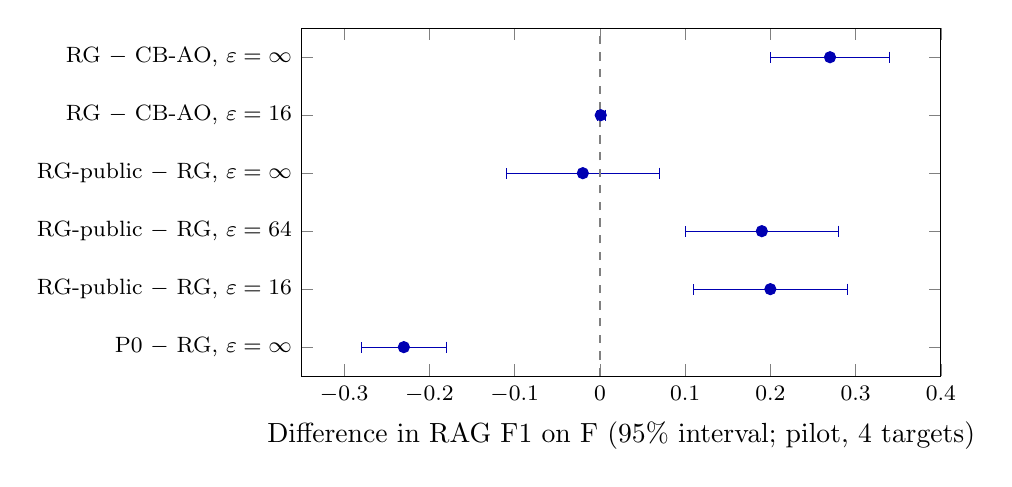
\begin{tikzpicture}
\begin{axis}[
  width=0.80\textwidth, height=6.0cm,
  xmin=-0.35, xmax=0.40, xlabel={Difference in RAG F1 on F (95\% interval; pilot, 4 targets)},
  ymin=0.5, ymax=6.5, ytick={1,2,3,4,5,6},
  yticklabels={{P0 $-$ RG, $\varepsilon=\infty$},{RG-public $-$ RG, $\varepsilon=16$},{RG-public $-$ RG, $\varepsilon=64$},{RG-public $-$ RG, $\varepsilon=\infty$},{RG $-$ CB-AO, $\varepsilon=16$},{RG $-$ CB-AO, $\varepsilon=\infty$}},
  y tick label style={font=\footnotesize}, x tick label style={font=\footnotesize},
]
\addplot[only marks, mark=*, blue!70!black,
  error bars/.cd, x dir=both, x explicit] coordinates {
  (0.27,6) += (0.07,0) -= (0.07,0)
  (0.001,5) += (0.006,0) -= (0.004,0)
  (-0.02,4) += (0.09,0) -= (0.09,0)
  (0.19,3) += (0.09,0) -= (0.09,0)
  (0.20,2) += (0.09,0) -= (0.09,0)
  (-0.23,1) += (0.05,0) -= (0.05,0)};
\draw[dashed, thick, gray] (axis cs:0,0.5) -- (axis cs:0,6.5);
\end{axis}
\end{tikzpicture}
\caption{Stage 1 utility differences (tuning data). At $\varepsilon=\infty$, grounded training gains about 0.27 F1 over the closed-book control and about 0.23 over the pretrained model. At $\varepsilon=64$ and 16, the DP-trained models fall back to about the utility of the pretrained model, and RG and CB-AO no longer differ.}\label{fig:pilot-utility}
\end{figure}

\paragraph{Leakage endpoints and projected precision.} Table~\ref{tab:pilot-proj} gives the descriptive pilot difference of each primary endpoint and its projected 99.3\% decision half-width. The projections use a normal approximation from the 4 pilot targets, scaled as $1/\sqrt{n}$, so they can be wrong by a factor of two. At 20 targets, the AUC endpoints would have half-widths of 0.15--0.24 against a margin of 0.05, so H1 and H3 would almost surely be inconclusive. The utility endpoints were already precise at 20 targets, except that their projections are optimistic, because the variation between article clusters and RG-public seeds does not shrink with the number of targets.

\begin{table}[htbp]
\centering
\caption{Stage 1 descriptive differences (estimate with 95\% interval; 4 targets per arm and budget; tuning data) and projected 99.3\% half-widths of the confirmation. Each difference has the orientation of Table~\ref{tab:conf-results}.}\label{tab:pilot-proj}
\small
\begin{tabular}{@{}llcc@{}}
\toprule
Endpoint & Pilot difference & \multicolumn{2}{c}{Projected half-width} \\
\cmidrule(l){3-4}
 & & 20 targets & 60 targets \\
\midrule
H1 Reference AUC, CB-AO $-$ RG ($\varepsilon=\infty$) & 0.19 [0.00, 0.75] & 0.24 & 0.14 \\
H1 utility, RG $-$ CB-AO ($\varepsilon=\infty$) & 0.27 [0.20, 0.34] & 0.043 & -- \\
H2 causal AUC, CB-AO $-$ RG, plain pass & 0.00 [0.00, 0.00] & 0.00 & -- \\
H2 causal AUC, CB-AO $-$ RG, release noise & $-0.12$ & 0.075 & 0.043 \\
H3 datastore AUC, RG $-$ CB-AO & 0.19 [0.00, 0.47] & 0.15 & 0.08 \\
H4 $R_{\mathrm{RG}}$ & 0.05 [0.00, 0.15] & 0.052 & 0.030 \\
H4 $D_{\mathrm{H4}}$ & 0.08 [0.00, 0.25] & 0.087 & 0.050 \\
H5 RG-public $-$ RG ($\varepsilon=\infty$) & $-0.02$ [$-0.11$, 0.07] & 0.054 & -- \\
H6 utility, RG $-$ CB-AO ($\varepsilon=16$, 10 targets) & 0.001 [$-0.003$, 0.007] & 0.004 & 0.004 \\
H6 Reference AUC, CB-AO $-$ RG ($\varepsilon=16$, 10 targets) & $-0.06$ [$-0.25$, 0.19] & 0.17 & 0.17 \\
H7 P0 $-$ RG ($\varepsilon=\infty$) & $-0.23$ [$-0.28$, $-0.18$] & 0.033 & -- \\
\bottomrule
\multicolumn{4}{@{}L{0.95\textwidth}@{}}{\footnotesize The H2 release-noise values are unpaired means over 4 targets per arm. The plain H2 pass sits at the ceiling, so its precision cannot be projected. ``--'': not projected, because cluster and seed variation does not shrink with targets. H6 keeps 10 targets in both columns.}
\end{tabular}
\end{table}

\paragraph{Consequences for the confirmation.} Three changes followed from the pilot. All of them were frozen in the Stage~2 protocol before any confirmation job ran.
\begin{enumerate}
  \item \textbf{60 targets at $\varepsilon=\infty$ instead of 20.} At 60 targets, the projected half-widths are 0.14 for H1, 0.08 for H3 and 0.030 and 0.050 for H4, so effects of the pilot's size become detectable for H1, H3 and H4, if the pilot estimates hold. More targets only narrow the intervals. Equivalence within $\pm0.05$ AUC would need roughly 170 (H3) to 450 (H1) targets, which our 124 final targets cannot provide.
  \item \textbf{H6 at $\varepsilon=16$ only.} The $\varepsilon=64$ jobs were dropped. This budget was a secondary, and in the pilot it behaved like $\varepsilon=16$. H6 stays primary and unchanged, with 10 targets.
  \item \textbf{H2 on the release-noise pass.} Without noise, the pre-registered H2 would measure the ceiling, not the arms. We therefore made the release-noise pass the H2 primary endpoint and kept the plain pass as a reported secondary with its own interval. H2 now measures leakage through noise-protected client releases, not through raw updates. This is a definition change after the pilot, not a tightening, so it is a new pre-registration. It also carries a selection risk, because we chose the endpoint after it showed a pilot difference between the arms. The confirmation uses only fresh final targets, so no pilot target contributes to H2.
\end{enumerate}
The CB-LM bridge is not run in the confirmation. The causal attack runs in each arm's frozen direction only.

\subsection{Stage 2: confirmation}\label{sec:res-stage2}

\paragraph{Execution checks.} All 146 confirmation jobs completed. Before the analysis, an integrity check verified every job without reading any endpoint value. In each world of a paired job, it checks six natural-question responses (three probes, with the target passage in and out of the library), three closed-book retention responses and 400 utility responses (300 on F and 100 on the public library). It also checks the 40 trials of each causal pass and the accounted budget of both worlds. At $\varepsilon=16$, both worlds of both arms accounted to $\varepsilon=16.0096$ over 51 steps in every pair, the same value as in the timing job, so RG and CB-AO are compared at the same budget. The grounded records of the target client have about 200 tokens on average and the CB-AO records about 60, all well within the 512-token limit, so no record was truncated. The answer tokens that carry the loss are the same in both arms. The difference in length is the passage in the context slot.

\paragraph{Computational cost.} Table~\ref{tab:conf-timing} gives the mean time of each type of confirmation job. RG training took about 40\% longer than CB-AO training, because its records are about three times as long, and each causal trial took about 5.1 seconds for RG and 4.2 seconds for CB-AO. The release noise added no measurable time. DP-SGD added 6\% (RG) and 14\% (CB-AO) to the training time. The measurements under DP took about 3.6 times longer than without DP in both arms, as in the timing job. A P0 job, which scores utility only, took 0.28~h, and an RG-public job took 0.16~h.

\begin{table}[htbp]
\centering
\caption{Mean time of one confirmation job (one causal direction, the frozen choice of each arm).}\label{tab:conf-timing}
\small
\begin{tabular}{@{}lrrrr@{}}
\toprule
 & \multicolumn{2}{c}{$\varepsilon=\infty$} & \multicolumn{2}{c}{$\varepsilon=16$} \\
\cmidrule(lr){2-3}\cmidrule(l){4-5}
Step & RG & CB-AO & RG & CB-AO \\
\midrule
FL training per world ($W_1$ / $W_0$) & 303 / 298 s & 218 / 214 s & 321 / 317 s & 249 / 244 s \\
Measurements per world ($W_1$ / $W_0$) & 275 / 300 s & 279 / 301 s & 996 / 1071 s & 997 / 1059 s \\
Causal attack: plain + release noise, 80 trials & 416 s & 342 s & 414 s & 342 s \\
\textbf{Total} & \textbf{0.45 h} & \textbf{0.38 h} & \textbf{0.87 h} & \textbf{0.81 h} \\
\bottomrule
\end{tabular}
\end{table}

\paragraph{Confirmatory results.} The analysis ran once on the completed confirmation, with the frozen attacker choices and decision rules. Table~\ref{tab:conf-results} gives the result of each primary hypothesis, and Figure~\ref{fig:conf-results} shows the estimates with their decision intervals. All intervals in this subsection are 99.3\% decision intervals from the target bootstrap, unless they are marked as 95\% intervals, and all margins are 0.05.

\begin{table}[tbp]
\centering
\small
\caption{Confirmation results (Stage 2; 60 fresh final targets at $\varepsilon=\infty$, 10 of them at $\varepsilon=16$; 99.3\% decision intervals; margin 0.05). Each difference is oriented so that a positive value is the direction of the hypothesis, except H5 and H7, which are utility differences against RG.}\label{tab:conf-results}
\begin{tabular}{@{}L{0.06\textwidth}L{0.34\textwidth}rL{0.14\textwidth}L{0.16\textwidth}c@{}}
\toprule
Hyp. & Difference & Estimate & Interval & Outcome & Claimed \\
\midrule
H1 & Reference AUC, CB-AO $-$ RG ($\varepsilon=\infty$) & 0.280 & [0.176, 0.368] & meaningful improvement & yes \\
 & utility, RG $-$ CB-AO (needs $\mathrm{lo}>-0.05$) & $+0.292$ & [0.237, 0.350] & acceptable & \\
H2 & causal AUC, CB-AO $-$ RG, release noise ($\varepsilon=\infty$) & $-0.052$ & [$-0.110$, 0.006] & inconclusive & no \\
 & secondary: plain pass, no noise & $+0.002$ & [$-0.007$, 0.017] & equivalent & -- \\
H3 & natural-question AUC, RG $-$ CB-AO ($\varepsilon=\infty$) & 0.350 & [0.230, 0.461] & meaningful improvement & yes \\
H4 & $R_{\mathrm{RG}}$ (F1) & $+0.006$ & [$-0.022$, 0.036] & equivalent & no \\
 & $D_{\mathrm{H4}}=R_{\mathrm{RG}}-R_{\mathrm{CB\text{-}AO}}$ (F1) & $+0.001$ & [$-0.046$, 0.047] & equivalent & \\
H5 & F1, RG-public $-$ RG ($\varepsilon=\infty$; needs $\mathrm{lo}>-0.05$) & $-0.096$ & [$-0.227$, 0.025] & not acceptable & no \\
H6 & F1, RG $-$ CB-AO ($\varepsilon=16$) & $+0.001$ & [$-0.006$, 0.012] & equivalent, not supported & no \\
 & Reference AUC, CB-AO $-$ RG ($\varepsilon=16$; needs $\mathrm{lo}>-0.05$) & $-0.10$ & [$-0.56$, 0.33] & no-worse not shown & \\
H7 & F1, P0 $-$ RG ($\varepsilon=\infty$) & $-0.211$ & [$-0.274$, $-0.144$] & RG meaningfully better & -- \\
\midrule
\multicolumn{6}{@{}L{0.96\textwidth}@{}}{\textbf{Cross-channel claim:} H1 supported and H3 supported, so the rule is met; a channel shift is claimed. H2 does not contribute.} \\
\bottomrule
\end{tabular}
\end{table}

\begin{figure}[tbp]
\centering
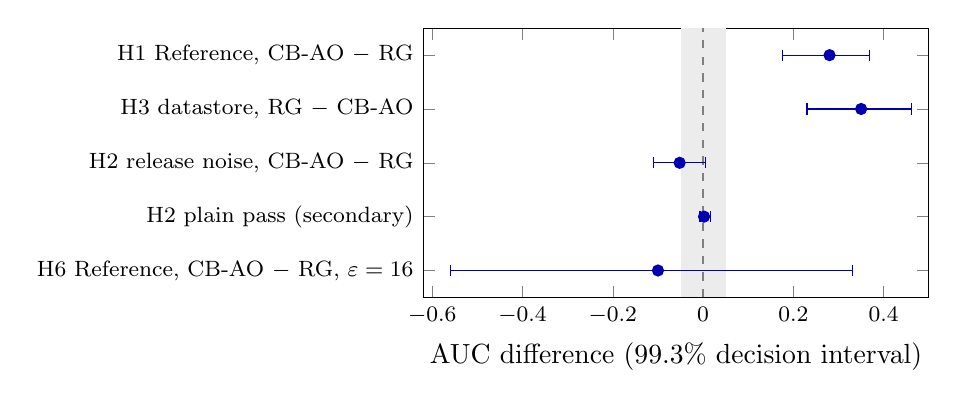
\begin{tikzpicture}
\begin{axis}[
  width=0.66\textwidth, height=5.0cm,
  xmin=-0.62, xmax=0.50, xlabel={AUC difference (99.3\% decision interval)},
  ymin=0.5, ymax=5.5, ytick={1,2,3,4,5},
  yticklabels={{H6 Reference, CB-AO $-$ RG, $\varepsilon=16$},{H2 plain pass (secondary)},{H2 release noise, CB-AO $-$ RG},{H3 datastore, RG $-$ CB-AO},{H1 Reference, CB-AO $-$ RG}},
  y tick label style={font=\footnotesize}, x tick label style={font=\footnotesize},
]
\fill[gray!15] (axis cs:-0.05,0.5) rectangle (axis cs:0.05,5.5);
\draw[dashed, thick, gray] (axis cs:0,0.5) -- (axis cs:0,5.5);
\addplot[only marks, mark=*, blue!70!black,
  error bars/.cd, x dir=both, x explicit] coordinates {
  (0.280,5) += (0.088,0) -= (0.104,0)
  (0.350,4) += (0.111,0) -= (0.120,0)
  (-0.052,3) += (0.058,0) -= (0.058,0)
  (0.002,2) += (0.015,0) -= (0.009,0)
  (-0.10,1) += (0.43,0) -= (0.46,0)};
\end{axis}
\end{tikzpicture}

\vspace{2mm}
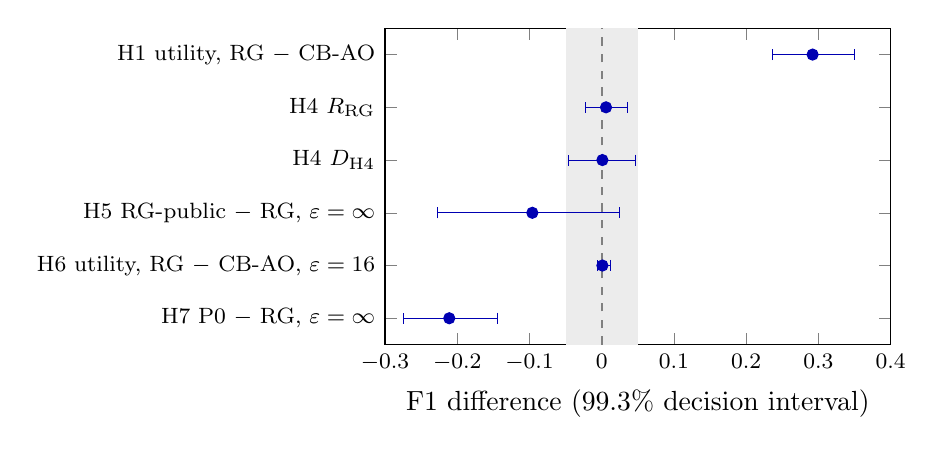
\begin{tikzpicture}
\begin{axis}[
  width=0.66\textwidth, height=5.6cm,
  xmin=-0.30, xmax=0.40, xlabel={F1 difference (99.3\% decision interval)},
  ymin=0.5, ymax=6.5, ytick={1,2,3,4,5,6},
  yticklabels={{H7 P0 $-$ RG, $\varepsilon=\infty$},{H6 utility, RG $-$ CB-AO, $\varepsilon=16$},{H5 RG-public $-$ RG, $\varepsilon=\infty$},{H4 $D_{\mathrm{H4}}$},{H4 $R_{\mathrm{RG}}$},{H1 utility, RG $-$ CB-AO}},
  y tick label style={font=\footnotesize}, x tick label style={font=\footnotesize},
]
\fill[gray!15] (axis cs:-0.05,0.5) rectangle (axis cs:0.05,6.5);
\draw[dashed, thick, gray] (axis cs:0,0.5) -- (axis cs:0,6.5);
\addplot[only marks, mark=*, blue!70!black,
  error bars/.cd, x dir=both, x explicit] coordinates {
  (0.292,6) += (0.058,0) -= (0.055,0)
  (0.006,5) += (0.030,0) -= (0.028,0)
  (0.001,4) += (0.046,0) -= (0.047,0)
  (-0.096,3) += (0.121,0) -= (0.131,0)
  (0.001,2) += (0.011,0) -= (0.007,0)
  (-0.211,1) += (0.067,0) -= (0.063,0)};
\end{axis}
\end{tikzpicture}
\caption{Confirmation results (Stage 2). Top: attack endpoints (AUC differences). Bottom: utility and retention endpoints (F1 differences). The grey band is the margin $\pm0.05$. Each difference has the orientation of Table~\ref{tab:conf-results}.}\label{fig:conf-results}
\end{figure}

\paragraph{H1: weights, record membership (supported).} The Reference AUC of CB-AO exceeded that of RG by 0.280 [0.176, 0.368]. The lower bound is above the margin, so the outcome is a meaningful improvement: under this attack, a grounded model reveals much less about which records it was trained on than a closed-book model. The utility condition holds by a wide gap, because RG answered 0.292 F1 [0.237, 0.350] better than CB-AO on F. The comparison uses each arm's own frozen Reference form, the record form for RG and the template form for CB-AO (Table~\ref{tab:choices}). For RG, this form won a pilot tie at 0.611 by the pre-registered tie rule. Every job recorded both forms, but only the frozen form decides H1.

\paragraph{H2: client updates (inconclusive).} Under release noise, the mean per-target causal AUC was higher for RG than for CB-AO, $D=-0.052$ [$-0.110$, 0.006]. The 95\% interval, [$-0.094$, $-0.010$], excludes zero, but the decision interval does not. H2 is therefore inconclusive: the data show neither that grounded training increases nor that it reduces leakage through noise-protected client updates. Without noise, both arms were again at the ceiling of the attack, and the secondary difference was equivalent to zero ($+0.002$ [$-0.007$, 0.017]). The H2 primary endpoint was chosen after the pilot (Section~\ref{sec:res-stage1}). It measures leakage through releases protected with $\sigma_{\mathrm{obs}}=1$, not through raw updates.

\paragraph{H3: datastore (supported).} With the F1 scorer in both arms, the natural-question AUC was higher for RG than for CB-AO by 0.350 [0.230, 0.461]. This is a meaningful increase in datastore detectability. A grounded model uses the retrieved passages more, so whether a passage is in the library shows more in its answers.

\paragraph{Cross-channel claim (holds).} H1 and H3 are both supported, so the pre-registered rule for a channel shift is met. With grounded training, record-membership leakage moves out of the weights and into the datastore channel. H2 is inconclusive and does not contribute to the claim.

\paragraph{H4: passage-fact retention (equivalent, not supported).} The mean retention of RG was $R_{\mathrm{RG}}=+0.006$ F1 [$-0.022$, 0.036], and its difference from CB-AO was $D_{\mathrm{H4}}=+0.001$ F1 [$-0.046$, 0.047]. Both intervals lie inside $\pm0.05$ F1, so both quantities are equivalent to zero within the margin, and H4 is not supported. The same probes detected deliberately memorized passage facts in the positive control (0.142 F1, Section~\ref{sec:res-stage0}), so this is an informative null result. In this setting, grounded training did not store the other facts of a training passage in the weights by more than 0.05 F1.

\paragraph{H5: public grounded training (acceptability not shown).} RG-public answered 0.096 F1 worse than private RG at $\varepsilon=\infty$, with interval [$-0.227$, 0.025]. The lower bound is below $-0.05$, so acceptable utility is not shown, and training on the private records helps answer quality in this setting. The pilot difference ($-0.02$) came from tuning data and did not carry over. Against RG at $\varepsilon=16$, RG-public answered 0.110 F1 better (95\% interval [0.014, 0.209]), which is consistent with the H6 result below.

\paragraph{H6: utility at an equal budget (not supported).} At $\varepsilon=16$, RG and CB-AO answered equally well: the F1 difference was $+0.001$ [$-0.006$, 0.012], equivalent within $\pm0.05$, so the utility part of H6 fails. The Reference AUC difference was $-0.10$ [$-0.56$, 0.33] on 10 targets. Its lower bound is below $-0.05$, so ``no worse leakage'' is not shown either. As in the pilot, DP-SGD at $\sigma=5.45$ removed the effect of fine-tuning in both arms.

\paragraph{H7: is fine-tuning needed? (RG meaningfully better).} The pretrained model answered 0.211 F1 worse than RG at $\varepsilon=\infty$ ($-0.211$ [$-0.274$, $-0.144$]). The upper bound is below $-0.05$, so RG is meaningfully better, and fine-tuning is needed for answer quality in this setting.

\paragraph{Scope of these results.} All results are measurements under the attacks of this study, not privacy guarantees. The $\varepsilon$ values cover only the accounted training releases (Section~\ref{sec:dp}). They do not cover the releases in answer to the crafted requests of the causal attack, the RAG outputs or the library. The setting is one model, one dataset and one FL configuration, and the datastore attacks are adaptations whose sensitivity, not strength, was validated in Stage~0.

% ===========================================================================
\section{Discussion}\label{sec:analysis}
% ===========================================================================

\subsection{What the validation establishes}\label{sec:readiness}

Stage~0 shows that each channel has a working instrument in this system, before any hypothesis is tested. The two natural-question scorers detected the target passage on the pretrained model with lower bounds of 0.854 and 0.837, well above the 0.70 bar, and they did so without verbatim probes. The verbatim baseline was weaker (AUC 0.75), and the calibrated gate withholds every verbatim probe at a benign cost of 4.4\%. A datastore attacker in a gated system therefore has to use natural questions, and these questions still work.

The retention probes detect deliberately memorized passage facts, but the 3-epoch control showed that learning a passage takes more exposure than one might assume: only 4 of 12 passages were learned after three central epochs at learning rate $10^{-4}$. Grounded federated training exposes a passage much less, with three rounds, one local epoch and the passage outside the loss. The positive control gives the null H4 result a known detection ability: the probes found 0.142 F1 of retention when a passage was memorized, and they found no retention beyond the 0.05 margin after grounded training.

The update-channel instrument was validated before this study, with a mean per-target AUC of 0.992 and no member/non-member pair in the wrong order. Its public threshold did not transfer to private batches (private FPR 0.165 at a 0.05 target), so we use a threshold-free per-target AUC as the H2 endpoint. The validation used closed-book records and no RAG. The pilot showed that the attack carries over to grounded records with the answer-only mask, provided that the server builds its request from the same template loss that the client trains on: the template direction reached 0.978 for RG, while the record direction failed (0.493). Without noise, the attack reached its ceiling in both arms, in the pilot and in the confirmation, so only release noise could separate them.

\subsection{What the pilot predicted and what held}\label{sec:pilot-discussion}

Two pilot findings shaped the confirmation, and both held. First, DP-SGD at our accounted budgets did not trade answer quality against leakage. It removed the fine-tuning effect: in the confirmation, RG and CB-AO at $\varepsilon=16$ answered equally well ($+0.001$ F1), and RG-public answered 0.110 F1 better than RG at $\varepsilon=16$. In this setting, a DP comparison of grounded and closed-book training compares two nearly pretrained models, so H6 could not be supported. A meaningful DP frontier needs a setup in which a DP-trained model can learn, for example parameter-efficient fine-tuning, larger batches or more records per client.

Second, the Reference attack is weak under the answer-only loss (tuning AUCs 0.46--0.61), while it is perfect under the full LM loss of the CB-LM bridge (1.000). Part of the weight leakage measured by earlier closed-book studies may thus come from the loss on the question tokens, which neither RG nor CB-AO trains on. The comparison of RG with CB-AO isolates the effect of the passage. With 60 targets, the H1 difference (0.280) was large enough to clear the margin in spite of the weak attack.

One pilot estimate did not hold. Public grounded training was close to private RG in the pilot ($-0.02$ F1 on 4 targets), but 0.096 F1 worse in the confirmation, so the confirmation could not show that public training is enough (H5). This is the reason that tuning data are never used as evidence.

\subsection{The channel shift and its mechanism}\label{sec:mechanism}

The measured pattern fits where the answer comes from. In CB-AO, the answer must come from the weights, so the client update must write the question--answer association into the weights. This is exactly the signal that the Reference attack reads. In RG, the answer is in the context, and the model learns to read it. The record-specific part of the update is smaller, and the Reference AUC fell by 0.280 (H1). The same reading skill makes the RAG system reveal what the library contains. When the target passage is in the library, an RG model's answers to its probes change more than a CB-AO model's answers, because the CB-AO model was trained to answer without context, and the natural-question AUC rose by 0.350 (H3). Grounding thus moved record-membership leakage from a place that FL exposes (the weights) to a place that the RAG deployment exposes (the library). It did not remove the leakage. This mechanism is our reading of the results. The study measures the two channels, not the mechanism itself.

The retention result narrows what ``in the weights'' means here. The answer-only mask does not remove the passage from the gradient (Section~\ref{sec:training-bg}), so grounded training could have stored the other facts of a training passage. It did not do so by more than 0.05 F1 (H4). Within this margin and under these probes, grounded training kept the passage's facts out of the model, and the passage stayed in the library, where the H3 attack finds it.

The update channel is different, because the malicious server does not depend on what the model stored. It crafts a request from the target's own loss and reads whether the returned gradient points in that direction. Both arms return a gradient that contains the target record when it is in the batch, so the attack reached its ceiling in both arms without noise. Training DP does not cover these crafted releases (Section~\ref{sec:dp}). Under release noise, the point estimate showed that RG leaked more than CB-AO ($-0.052$), and the 95\% interval excluded zero, but the decision interval did not. A plausible cause is that the target's gradient in RG depends on the passage as well as the answer: a grounded record is about three times as long as its CB-AO counterpart, while the loss tokens are the same (Section~\ref{sec:res-stage2}). The study cannot decide this. What it does show is that the update channel stays exposed in both arms, whatever the training format, and that it needs its own defense.

\subsection{What the results do not show}\label{sec:falsify}

\begin{itemize}
  \item \textbf{H1 does not show that grounded weights are private.} H1 compares each arm under its own frozen Reference form. It shows that a grounded model reveals less record membership to this attack than a closed-book model. It does not show that a stronger or differently tuned attack would fail.
  \item \textbf{H4 does not show that no passage fact is stored.} Equivalence means that retention stayed within $\pm0.05$ F1 under three closed-book probes per passage. Smaller effects, other facts and extraction by a stronger attacker remain possible.
  \item \textbf{H2 shows no difference in either direction.} The point estimate shows more leakage for RG, but the decision interval includes zero, and the primary endpoint was chosen after the pilot, so the result must not be read as ``RG leaks more through updates''. It must not be read as ``no change'' either, because the interval is wider than the margin on the harm side.
  \item \textbf{H5 does not show that public training is useless.} It shows that acceptable utility relative to private RG could not be established. Public grounded training still answered better than RG at $\varepsilon=16$.
  \item \textbf{H6 does not compare two learning models.} Both DP-trained arms answered like the pretrained model, so H6 says nothing about grounded versus closed-book training under a DP budget at which the model learns.
\end{itemize}

\subsection{Limitations}\label{sec:scope}

\begin{itemize}
  \item The setting is narrow: one model (Qwen2.5-0.5B-Instruct), one dataset (SQuAD) and one FL setting with four clients and three rounds. We make no general claims.
  \item All results are measurements under the attacks of this study. They are not privacy guarantees.
  \item SQuAD is public. It cannot show that a fact was absent from pretraining. We treat it as a simulated private benchmark.
  \item The datastore attacks are adaptations. Stage~0 validates only their sensitivity. Stronger attackers can exist.
  \item H1 compares each arm under its own frozen Reference form (record form for RG, template form for CB-AO). This is the pre-registered rule, but a comparison at a common form was not part of the decision.
  \item The $\varepsilon$ values are large because the accountant is conservative. They are comparable between arms, and they cover only the accounted training releases. They do not cover the crafted-request releases, the RAG outputs or the library. There is no end-to-end $\varepsilon$.
  \item RG training uses the gold passage (oracle context), not a retrieved passage.
  \item All attacks are membership inference. A low membership AUC does not show that the model resists extraction.
  \item The causal validation had 20 non-members per target, so it cannot estimate the TPR at a 1\% FPR \citep{carlini2022first}.
  \item The H2 primary endpoint was chosen after the pilot, when the release-noise pass showed a difference between the arms. Fresh targets and the reported plain-pass secondary limit, but do not remove, this selection risk.
  \item DP-SGD at our budgets erased fine-tuning in the pilot and in the confirmation. The DP results therefore describe nearly pretrained models. The confirmation ran only $\varepsilon=16$, with 10 targets, so the H6 Reference interval is wide.
  \item At 60 targets, the AUC endpoints are too imprecise to show equivalence within $\pm0.05$ AUC (Section~\ref{sec:res-stage1}). An AUC difference that is not shown is therefore not evidence that there is no difference.
  \item We claim no new defense mechanism.
\end{itemize}

% ===========================================================================
\section{Conclusion}\label{sec:conclusion}
% ===========================================================================

We built a controlled study of where private information goes when federated clients train an LLM to answer from supplied passages instead of closed-book. The four-cell design crosses grounding, training membership and library membership. The arms differ only in the context slot, and they are compared at matched, accounted DP budgets. A pre-registered three-stage protocol validated the instruments, tuned the attacker on validation data and tested seven hypotheses on 60 fresh targets. The study yields these results:
\begin{itemize}
  \item Of eleven published MIAs adapted to federated fine-tuning, most gave no useful membership decisions in this environment. The Reference attack on the weights and an active-server attack on the client updates carry the study, together with natural-question attacks on the library (pooled AUC 0.902 and 0.887 on the pretrained model, where a calibrated gate blocks every verbatim probe).
  \item Grounded training lowered record-membership leakage through the weights (Reference AUC difference, closed-book minus grounded, 0.280 [0.176, 0.368]) and improved the RAG answers by 0.292 F1 [0.237, 0.350].
  \item Grounded training made library documents easier to detect (natural-question AUC $+0.350$ [0.230, 0.461]). With H1, this meets the pre-registered rule for a channel shift: leakage moved from the weights to the datastore.
  \item Grounded training did not store the passage's other facts in the weights by more than 0.05 F1 ($R_{\mathrm{RG}}=+0.006$ [$-0.022$, 0.036]), although the same probes detect deliberate memorization (0.142 F1).
  \item A malicious server that sends a crafted, architecture-preserving request reached the ceiling of its attack in both arms without noise. Under release noise, the comparison of the arms was inconclusive ($-0.052$ [$-0.110$, 0.006]).
  \item DP-SGD at $\varepsilon=16$ returned both arms to the answer quality of the pretrained model. Without DP, fine-tuning was needed: grounded training answered 0.211 F1 better than the pretrained model, and public grounded training did not reach acceptable utility relative to private grounded training.
\end{itemize}
Grounded training therefore moves leakage between channels rather than removing it. A federated RAG deployment that trains with retrieved context protects the weights better, but it must protect its library and its client updates separately.

% ===========================================================================
\section{Further Studies}\label{sec:further}
% ===========================================================================

The completed three-stage study gives a channel-by-channel map of leakage under grounded and closed-book federated training. The following studies build on that map:
\begin{enumerate}
  \item \textbf{Defend the datastore channel.} Grounding moved leakage into the library, so the next step is a defense for that channel. Candidates are access control on the library and a retrieval gate that also covers natural-question probes, not only verbatim ones. The verbatim-overlap gate of this study is a starting point, because its benign cost is known (4.4\%), and our calibration of Mirabel \citep{choi2025mirabel} showed the cost of a detector that is too strict for this system (Section~\ref{sec:battery}). The defense should be evaluated with the same attack battery, the same four cells and the same utility measures, so that a gain on the library is not paid for in the weights.
  \item \textbf{Protect the client updates.} The active-server attack reached its ceiling in both arms without noise. Release noise with a range of $\sigma_{\mathrm{obs}}$, secure aggregation and a client-side check of the received model are candidates. More targets would also settle whether grounded training leaks more through noise-protected updates.
  \item \textbf{Make DP training useful.} At our budgets, DP-SGD erased the fine-tuning effect. A DP comparison of grounded and closed-book training needs a setup in which a DP-trained model learns, such as parameter-efficient fine-tuning with LoRA adapters, larger batches or more records per client, with its own pilot.
  \item \textbf{Generalize the setting.} A broader study needs other model sizes and families, other datasets with controlled private facts, non-IID clients with different data sizes, and more training exposure (more rounds or local epochs). It also needs stronger attacks on the weights, such as LiRA with shadow models \citep{carlini2022first}, and low-FPR operating points with more non-members per target.
  \item \textbf{Use retrieved context in training.} RG training used the gold passage. A study with retrieved top-$k$ context and distractors, as in RAFT \citep{zhang2024raft}, would show whether the channel shift holds with an imperfect retriever.
  \item \textbf{Add an extraction test.} Membership AUC and closed-book retention do not show that facts are absent from the weights. A controlled extraction test with synthetic secrets (canaries) is necessary for any stronger claim that grounded training keeps facts out of the model.
  \item \textbf{Tighten the accounting and test adaptive attackers.} A participation-based accountant would give smaller $\varepsilon$ values for the same noise. Each attacker in this study knows the candidate but not the defense. An attacker that knows the training format, the gate or the release noise is the next test for any defense from items~1 and~2.
\end{enumerate}

\bibliographystyle{plainnat}
\bibliography{references}

\end{document}
